\documentclass[
%   draft,
  a4paper,
%   titlepage,
  onecolumn,
%  twocolumn,
  12pt,
  ]%
% {scrartcl}%
{article}%


\usepackage[utf8x]{inputenc} 
%\usepackage[utf8]{inputenc} % codificação deste ficheiro em UTF-8 

\usepackage[T1]{fontenc} % necessário para que os caracteres acentuados possam ser considerados como um só bloco ( efeito colaterar: necessita de uma fonte que não a CM para não ficar com um aspecto aceitável)

%% precisa ser carregado um outro tipo de letra por causa do efeito colateral do pacote T1:
\usepackage{lmodern} % Fonte "Latin Modern" - A solução óptima para fontes latinas (resolve o problema do T1)
% \usepackage{times}   % Fonte "Times"


\usepackage{textcomp} % caracteres extra - símbolo do euro por exemplo

% \usepackage[portuguese]{babel} % tradução portuguesa
% \newcommand{\referencesname}{Bibliografia}
\newcommand{\referencesname}{References}


%%%%%%%%%% Packages


\usepackage[pdftex]{graphicx} % figuras 
% \usepackage{subfigure} % subfiguras ( a,b,... )
% \usepackage{wrapfig} % figuras ao lado de texto


\usepackage{array} % mais opções nas tabelas (m{width}, b{width}, ...)
\setlength{\extrarowheight}{1pt} % extra espaço entre as linhas das tabelas
% \usepackage{multirow} % tabelas com células multilinha

\usepackage{fancyhdr} % Estilo de página

% \usepackage{listings} % Highlight de código fonte
% \renewcommand{\lstlistingname}{Listagem} % tradução para português (referente ao package listings)
% \renewcommand{\lstlistlistingname}{Listagens} % tradução para português (referente ao package listings)

\usepackage[usenames,hyperref,pdftex%
 ,svgnames%
 ,x11names%
 ,dvipsnames%
%  ,cmyk
 ]{xcolor} % Utilização de cores
\usepackage{multicol}


\usepackage[left=2.3cm,right=2.3cm,top=2.4cm]{geometry} % Margins

% \usepackage{setspace} % spacing between lines (\singlespacing, \onehalfspacing, ...)

% math packages by AMS
\usepackage{amsmath} % main one
% \usepackage{amsfonts}
% \usepackage{amssymb}


% \usepackage{moreverb} % more verbatim options (boxedverbatim)
\usepackage{fancyvrb} % more verbatim options 

% \usepackage{lipsum}


% \usepackage{tikz}
% Optional tikz libraries
% \usetikzlibrary{arrows}


\usepackage[square, comma, sort&compress]{natbib}

\setcitestyle{super,comma}

% \usepackage[protrusion=true,expansion=true]{microtype}
\usepackage[protrusion=true,expansion=true,stretch=10,shrink=10]{microtype} % micro-typographic extensions of pdfTEX (gets high quality text compostion)

\usepackage[
      pdftex,             %driver
      colorlinks=true,    %no frame around URL
      urlcolor=DarkGreen!70!Black,    %no colors
%       menucolor=black,    %no colors
      linkcolor=black,    %no colors
%       pagecolor=black,    %no colors
      citecolor=DarkGreen!70!Black,    %no colors
      bookmarks=true,    %tree-like TOC
      bookmarksopen=true,    %expanded when starting
      bookmarksnumbered=true, %Put section numbers in bookmarks
      hyperfootnotes=true,    %no referencing of footnotes, does not compile
      pdfpagemode=UseOutlines,    %show the bookmarks when starting the pdf viewer
      plainpages=false, %solve problem ``destination with the same identifier'' warning
      pdfpagelabels %solve problem ``destination with the same identifier'' warning
]{hyperref} % fazer hyperlinks (usar como último ``usepackage'')


% \usepackage[style=altlist,hypertoc,hyper,number=page]{glossary}


% \usepackage{pdfpages}

 \usepackage[]{todonotes}
% \usepackage[disable]{todonotes}

\usepackage{xifthen}
\usepackage{csvsimple}



\newcommand{\tab}{\hspace*{2em}}

%Text subscript
\usepackage{fixltx2e}

% Matrizes
\usepackage{amsmath}

%rename defaults

\renewcommand{\figurename}{Figura}
\renewcommand{\contentsname}{Tabela de conteúdos}
\renewcommand{\abstractname}{Introdução}
\renewcommand{\refname}{Referências}


%Figure side by side

\usepackage{subfig}

%force float position
\usepackage{float}
\usepackage[section]{placeins}

\makeatletter
\AtBeginDocument{%
  \expandafter\renewcommand\expandafter\subsection\expandafter{%
    \expandafter\@fb@secFB\subsection
  }%
}
\makeatother
%%%%%%%%%%%%%%%%%%%%%%%%%%%%%%%%%%%%%%%%%%%%%%%%%%%%%%%%%%%%%%%% 


% Ifenização
%\hyphenation{apli-ca-ção cons-tru-ção}% ...

%%%%%%%%%%%%%%%%%%%%%%%%%%%%%%%%%%%%%%%%%%%%%%%%%%%%%%%%%%%%%%%%
%Parametros de exibicao de codigo
\usepackage{listings}
\usepackage{color}

\definecolor{mygreen}{rgb}{0,0.6,0}
\definecolor{mygray}{rgb}{0.5,0.5,0.5}
\definecolor{mymauve}{rgb}{0.58,0,0.82}

\lstset{ %
  backgroundcolor=\color{white},   % choose the background color; you must add \usepackage{color} or \usepackage{xcolor}
  basicstyle=\footnotesize,        % the size of the fonts that are used for the code
  breakatwhitespace=false,         % sets if automatic breaks should only happen at whitespace
  breaklines=true,                 % sets automatic line breaking
  captionpos=b,                    % sets the caption-position to bottom
  commentstyle=\color{mygreen},    % comment style
  deletekeywords={...},            % if you want to delete keywords from the given language
  escapeinside={\%*}{*)},          % if you want to add LaTeX within your code
  extendedchars=true,              % lets you use non-ASCII characters; for 8-bits encodings only, does not work with UTF-8
  frame=single,                    % adds a frame around the code
  keepspaces=true,                 % keeps spaces in text, useful for keeping indentation of code (possibly needs columns=flexible)
  keywordstyle=\color{blue},       % keyword style
  language=Matlab,                 % the language of the code
  morekeywords={*,...},            % if you want to add more keywords to the set
  numbers=left,                    % where to put the line-numbers; possible values are (none, left, right)
  numbersep=5pt,                   % how far the line-numbers are from the code
  numberstyle=\tiny\color{mygray}, % the style that is used for the line-numbers
  rulecolor=\color{black},         % if not set, the frame-color may be changed on line-breaks within not-black text (e.g. comments (green here))
  showspaces=false,                % show spaces everywhere adding particular underscores; it overrides 'showstringspaces'
  showstringspaces=false,          % underline spaces within strings only
  showtabs=false,                  % show tabs within strings adding particular underscores
  stepnumber=2,                    % the step between two line-numbers. If it's 1, each line will be numbered
  stringstyle=\color{mymauve},     % string literal style
  tabsize=2,                       % sets default tabsize to 2 spaces
  title=\lstname                   % show the filename of files included with \lstinputlisting; also try caption instead of title
  %inputencoding=ansinew
}


%%%%%%%%%%%%%%%%%%%%%%%%%%%%%%%%%%%%%%%%%%%%%%%%%%%%%%%%%%%%%%%%

%% Criação de comandos:


\newcommand{\note}[1]{{\sffamily \slshape \textcolor{red}{#1}}}

\colorlet{FPathColor}{Sepia}
\colorlet{CmdColor}{blue}
\colorlet{CmdRuleColor}{LightSteelBlue}
\colorlet{FileTextColor}{DarkGreen}
\colorlet{FuncColor}{DeepPink4}
\CustomVerbatimCommand{\FPath}{Verb}{formatcom=\color{FPathColor},fontsize=\normalsize}
\CustomVerbatimCommand{\Cmd}{Verb}{formatcom=\color{CmdColor},fontsize=\normalsize}
\CustomVerbatimCommand{\FText}{Verb}{formatcom=\color{FileTextColor},fontsize=\normalsize}
\CustomVerbatimCommand{\Func}{Verb}{formatcom=\color{FuncColor},fontsize=\normalsize}
\DefineVerbatimEnvironment%
  {Command}{Verbatim}
  {formatcom=\color{CmdColor},frame=single,rulecolor=\color{CmdRuleColor},fontsize=\normalsize}
\DefineVerbatimEnvironment%
  {FileText}{Verbatim}
  {formatcom=\color{FileTextColor},fontsize=\normalsize}


% % Authors:


\newcommand{\MYauthor}{João Toscano Ferreira}
\newcommand{\MYnumber}{2010144652}

\newcommand{\MYauthorII}{José Pedro Medeiros} % Can be commented
\newcommand{\MYnumberII}{2010129934} % Can be commented




% % Titles:
\newcommand{\MYtitle}{Navegação de Robôs Móveis
Utilização de Campos de Potencial para Navegação de Robôs Móveis.}
\newcommand{\MYsubtitle}{Labwork - 5} % Can be empty


% % Course

\newcommand{\MYcoursename}{Sistemas Robóticos e Robótica Móvel}
\newcommand{\MYcourseyear}{2015/2016}


% % PDF infos

\newcommand{\MYkeywords}{} % Can be empty
\newcommand{\MYsubject}{} % Can be empty


%%%%%%%%%%%%%%%%%%%%%%%%%%%%%%%%%%%%%%%%%%%%%%%%%%%%%%%%%%
%%%%%%%%%%%%%%%%%%%%%%%%%%%%%%%%%%%%%%%%%%%%%%%%%%%%%%%%%%%%%%%%%%%%%%%%%%%%%%%%%%%%%%%%%%%%%%%%%%%%%%%%%%%%%%%%%%%
%%%%%%%%%%%%%%%%%%%%%%%%%%%%%%%%%%%%%%%%%%%%%%%%%%%%%%%%%%%%%%%%%%%%%%%%%%%%%%%%%%%%%%%%%%%%%%%%%%%%%%%%%%%%%%%%%%%%%%%%%%%%%%%%

%% Document format

%% Fancy Headers
\lhead{
\includegraphics[width=2cm]{logo_deec.pdf}}
\chead{\sc\footnotesize Universidade de Coimbra\\
Faculdade de Ciências e Tecnologia\\
Departamento de Engenharia Electrotécnica e de Computadores}
\rhead{
\includegraphics[width=0.8cm]{logo_fctuc.pdf}}
\setlength{\headheight}{43pt}

% Title
\title{{\large\MYcoursename\ -- \MYcourseyear}\\[2mm]
{\MYtitle}
\ifthenelse{\equal{\MYsubtitle}{}}
{\vspace*{1mm}}   {\\{\large\MYsubtitle}\vspace*{1mm}}
}

% Author / Number
\author{%
\MYauthor\\{\normalsize \href{mailto:a\MYnumber@alunos.deec.uc.pt}{\MYnumber}}
\ifthenelse{\isnamedefined{MYauthorII}}
{\and\MYauthorII\\{\normalsize \href{mailto:a\MYnumberII@alunos.deec.uc.pt}{\MYnumberII}}}    {}
\ifthenelse{\isnamedefined{MYauthorIII}}
{\and\MYauthorIII\\{\normalsize \href{mailto:a\MYnumberIII@alunos.deec.uc.pt}{\MYnumberIII}}}   {}
}

% Version / Date
\date{%
% \normalsize \today
\mbox{}
}

%%%%%%%%%%%%%%%%%%%%%%%%%%%%%%%%%%%%%%%%%%%%%%%%%%%%%%%%%%%%%%%%


%% PDF definitions:

\hypersetup{%
   pdftitle=\MYtitle,%
   pdfauthor=\MYauthor,%
%    pdfcreator=,%
   pdfkeywords= {\MYkeywords},%
%    pdfproducer=,%
   pdfsubject= \MYsubject%
} % informações do pdf (pacote hyperref)

\pdfinfo{
/Title	(\MYtitle)
/Author (\MYauthor)
/Keywords (\MYkeywords)
} % informações do pdf

%%%%%%%%%%%%%%%%%%%%%%%%%%%%%%%%%%%%%%%%%%%%%%%%%%%%%%%%%%%%%%%%
%%%%%%%%%%%%%%%%%%%%%%%%%%%%%%%%%%%%%%%%%%%%%%%%%%%%%%%%%%%%%%%%
%%%%%%%%%%%%%%%%%%%%%%%%%%%%%%%%%%%%%%%%%%%%%%%%%%%%%%%%%%%%%%%%
%%%%%%%%%%%%%%%%%%%%%%%%%%%%%%%%%%%%%%%%%%%%%%%%%%%%%%%%%%%%%%%%
%%%%%%%%%%%%%%%%%%%%%%%%%%%%%%%%%%%%%%%%%%%%%%%%%%%%%%%%%%%%%%%%
%%%%%%%%%%%%%%%%%%%%%%%%%%%%%%%%%%%%%%%%%%%%%%%%%%%%%%%%%%%%%%%%
%%%%%%%%%%%%%%%%%%%%%%%%%%%%%%%%%%%%%%%%%%%%%%%%%%%%%%%%%%%%%%%%
%%%%%%%%%%%%%%%%%%%%%%%%%%%%%%%%%%%%%%%%%%%%%%%%%%%%%%%%%%%%%%%%
%%%%%%%%%%%%%%%%%%%%%%%%%%%%%%%%%%%%%%%%%%%%%%%%%%%%%%%%%%%%%%%%
%%%%%%%%%%%%%%%%%%%%%%%%%%%%%%%%%%%%%%%%%%%%%%%%%%%%%%%%%%%%%%%%
%%%%%%%%%%%%%%%%%%%%%%%%%%%%%%%%%%%%%%%%%%%%%%%%%%%%%%%%%%%%%%%%
%%%%%%%%%%%%%%%%%%%%%%%%%%%%%%%%%%%%%%%%%%%%%%%%%%%%%%%%%%%%%%%%
%%%%%%%%%%%%%%%%%%%%%%%%%%%%%%%%%%%%%%%%%%%%%%%%%%%%%%%%%%%%%%%%
%%%%%%%%%%%%%%%%%%%%%%%%%%%%%%%%%%%%%%%%%%%%%%%%%%%%%%%%%%%%%%%%
%%%%%%%%%%%%%%%%%%%%%%%%%%%%%%%%%%%%%%%%%%%%%%%%%%%%%%%%%%%%%%%%
%%%%%%%%%%%%%%%%%%%%%%%%%%%%%%%%%%%%%%%%%%%%%%%%%%%%%%%%%%%%%%%%
%%%%%%%%%%%%%%%%%%%%%%%%%%%%%%%%%%%%%%%%%%%%%%%%%%%%%%%%%%%%%%%%
%%%%%%%%%%%%%%%%%%%%%%%%%%%%%%%%%%%%%%%%%%%%%%%%%%%%%%%%%%%%%%%%
%%%%%%%%%%%%%%%%%%%%%%%%%%%%%%%%%%%%%%%%%%%%%%%%%%%%%%%%%%%%%%%%
%%%%%%%%%%%%%%%%%%%%%%%%%%%%%%%%%%%%%%%%%%%%%%%%%%%%%%%%%%%%%%%%
%%%%%%%%%%%%%%%%%%%%%%%%%%%%%%%%%%%%%%%%%%%%%%%%%%%%%%%%%%%%%%%%
%%%%%%%%%%%%%%%%%%%%%%%%%%%%%%%%%%%%%%%%%%%%%%%%%%%%%%%%%%%%%%%%
%%%%%%%%%%%%%%%%%%%%%%%%%%%%%%%%%%%%%%%%%%%%%%%%%%%%%%%%%%%%%%%%
%%%%%%%%%%%%%%%%%%%%%%%%%%%%%%%%%%%%%%%%%%%%%%%%%%%%%%%%%%%%%%%%
%%%%%%%%%%%%%%%%%%%%%%%%%%%%%%%%%%%%%%%%%%%%%%%%%%%%%%%%%%%%%%%%
%%%%%%%%%%%%%%%%%%%%%%%%%%%%%%%%%%%%%%%%%%%%%%%%%%%%%%%%%%%%%%%%
%%%%%%%%%%%%%%%%%%%%%%%%%%%%%%%%%%%%%%%%%%%%%%%%%%%%%%%%%%%%%%%%
%%%%%%%%%%%%%%%%%%%%%%%%%%%%%%%%%%%%%%%%%%%%%%%%%%%%%%%%%%%%%%%%
%%%%%%%%%%%%%%%%%%%%%%%%%%%%%%%%%%%%%%%%%%%%%%%%%%%%%%%%%%%%%%%%
%%%%%%%%%%%%%%%%%%%%%%%%%%%%%%%%%%%%%%%%%%%%%%%%%%%%%%%%%%%%%%%%
%%%%%%%%%%%%%%%%%%%%%%%%%%%%%%%%%%%%%%%%%%%%%%%%%%%%%%%%%%%%%%%%
%%%%%%%%%%%%%%%%%%%%%%%%%%%%%%%%%%%%%%%%%%%%%%%%%%%%%%%%%%%%%%%%
%%%%%%%%%%%%%%%%%%%%%%%%%%%%%%%%%%%%%%%%%%%%%%%%%%%%%%%%%%%%%%%%
%%%%%%%%%%%%%%%%%%%%%%%%%%%%%%%%%%%%%%%%%%%%%%%%%%%%%%%%%%%%%%%%
%%%%%%%%%%%%%%%%%%%%%%%%%%%%%%%%%%%%%%%%%%%%%%%%%%%%%%%%%%%%%%%%
%%%%%%%%%%%%%%%%%%%%%%%%%%%%%%%%%%%%%%%%%%%%%%%%%%%%%%%%%%%%%%%%

\graphicspath{ {img/} } % Pasta das Imagens



\begin{document}

\maketitle
\thispagestyle{fancyplain}

%%%%%%%%%%%%%%%%%%%%%%%%%%%%%%%%%%%%%%%%%%%%%%%%%%%%%%%%%%%%%%%%%%%%%%%%%
%% Introdução
 \begin{abstract} %


\indent \\ \indent Com este trabalho pretende-se dar à plataforma móvel a capacidade de navegar de um ponto inicial a um ponto objectivo, percorrendo um mapa que poderá incluir obstáculos. Para se atingir este objectivo foram utilizados campos de pontecial. \\ \indent Os campos de potencial são utilizados em robótica móvel para evitar que as plataformas móveis colidam com obstáculos. O princípio de funcionamento destes campos é simples, no local do ponto objectivo é colocada uma carga atractiva que gera um campo de potencial que vai atrair a plataforma móvel, por outro lado no locais do mapa em que são detectados obstáculos (durante o percurso) é colocada uma carga repulsiva que gera um campo de potencial que irá repelir a plataforma. \\ \indent Finalmente, somando os dois campos de pontencial (repulsivo e atractivo) que ajudará a plataforma a navegar afastando-a dos obstáculos e aproximando-a para o ponto objectivo.








 \end{abstract}

%%%%%%%%%%%%%%%%%%%%%%%%%%%%%%%%%%%%%%%%%%%%%%%%%%%%%%%%%%%%%%%%%%%%%%%%%
%% Inicio
\section{Execução do Simulador - GUI}
\indent \\ \indent  Para correr o simulador, o utilizador deve correr o comando \textbf{\textit{Simulador}} no Matlab, este comando vai correr a interface gráfica por nós desenvolvida da qual o código correspondente se encontra no ficheiro \textit{Simulador.m}.
\\

%-------------------------------------------------------------------------
\subsection{Simulação da plataforma}

 \indent \\  \indent A interface gráfica sofreu alterações relativamente
ao trabalho anterior dado que foi introduzida navegação ponto a ponto e ainda que foram introduzidos os campos de potenial. É apresentada a figura \ref{fig:fig1} que ilustra o novo ambiente para este
trabalho, incluindo o novo mapa de campos de potencial.
\\  \indent  O utilizador deverá escolher entre navegação reactiva ou navegação ponto a ponto. No caso de escolha de navegação ponto a ponto, o utilizador deverá inicalmente clicar em \textbf{- iniciar navegação}, posteriormente escolher o ponto objectivo \textbf{(pressionando ENTER)} e de seguida  deve clicar no mapa na posição desejada para o início da navegação, clicando uma segunda vez para a orientação pretendida e a navegação irá começar automaticamente .\\  \indent No caso de o utilizador escolher navegação reactiva para que este possa escolher a posição e orientação do robot basta escolher no simulador \textbf{- Iniciar Simulação -> Escolher ponto e orientação. } e de seguida clicar no mapa na posição desejada, clicando uma segunda vez para a orientação pretendida, o utilizador pode também optar por uma posição predefinida. É dada a oportunidade ao utilizador de definir o tempo de simulação desejado.  \\ \indent Para iniciar a simulação basta ao utilizador clicar no botão \textbf{- iniciar comportamento reactivo}. \\ \indent Isto pode ser visualizado na figura~\ref{fig:fig1}.




\begin{figure}[h]
\centering

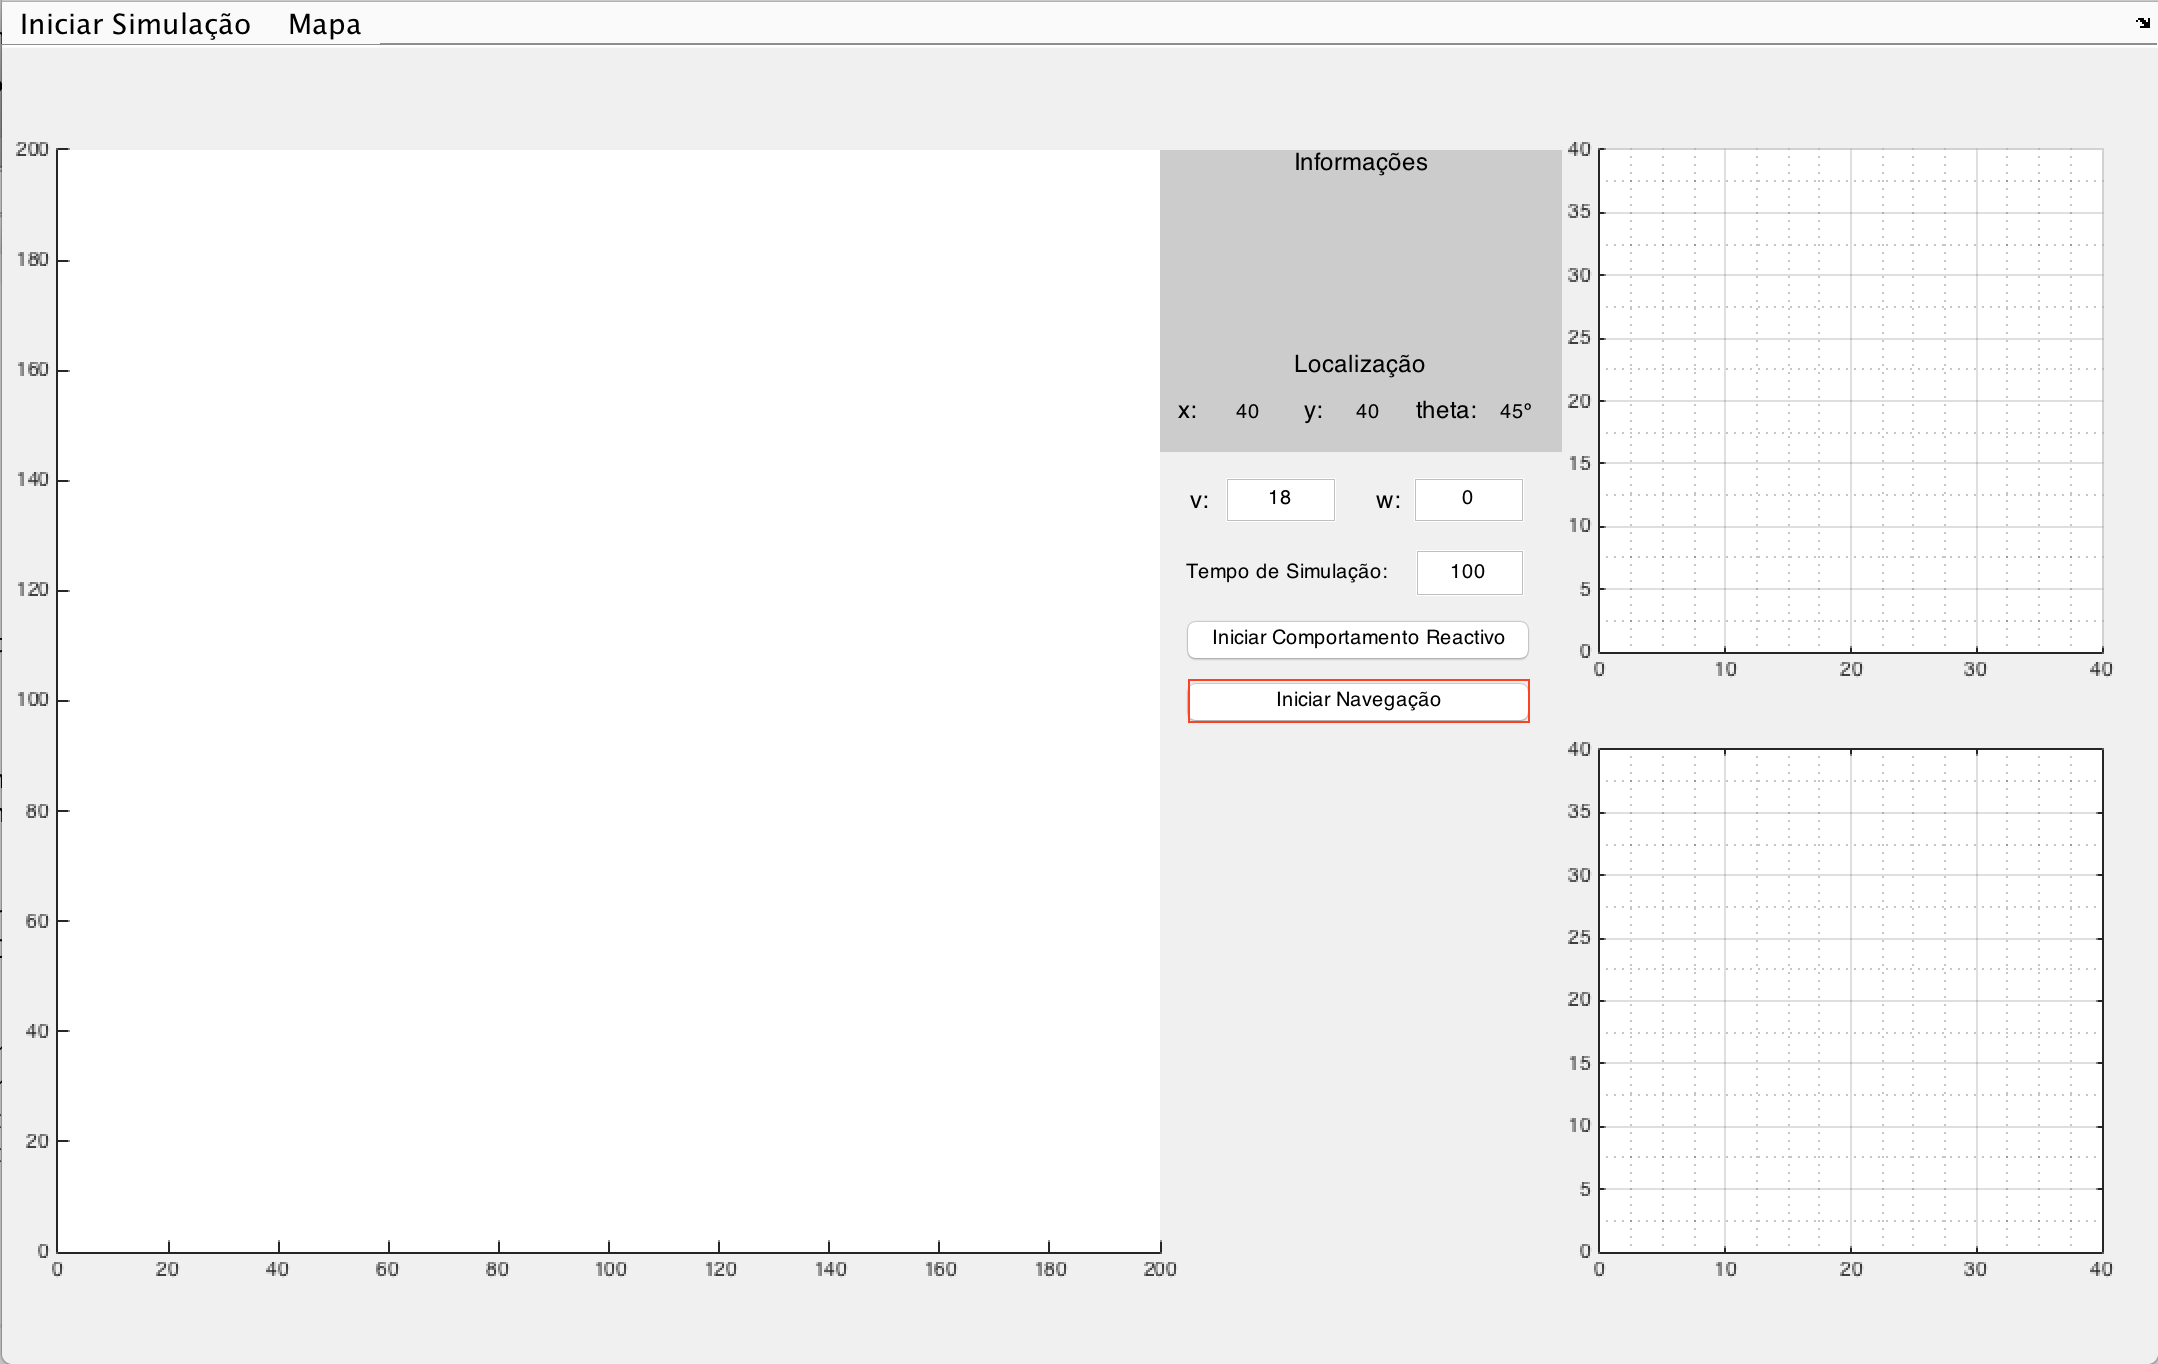
\includegraphics[width=90mm,scale=0.3]{img1.png}
\caption{Captura do Simulador no momento de escolha da posição e orientação inicial. }\label{fig:fig1}
\end{figure}



%-------------------------------------------------------------------------
\subsection{Definição do mapa de obstáculos}
 \indent \\ \indent O simulador oferece ao utilizador possibilidade de desenhar obstáculos, criar e guardar mapas assim como permite a possibilidade de os carregar no futuro. \\ \indent Para que o utilizador possa criar obstáculos este deve escolher \textbf{- Mapa -> Criar obstáculo. } e de seguida deve clicar no mapa com o botão esquerdo do racto por forma a definir os diversos vértices do polígono e de seguida deverá clicar com o botão direito do rato definindo o último vértice e finalizando assim o preenchimento do obstáculo. Para carregar um mapa o utilizador seleciona \textbf{- Mapa -> Carregar mapa. }, o mesmo é válido para guardar o mapa devendo o utilizador selecionar \textbf{- Mapa -> Guardar mapa. } e ainda para quando o utilizador pretende limpar o mapa \textbf{- Mapa -> Limpar mapa. }.  \\


\begin{figure}[ht]
\centering
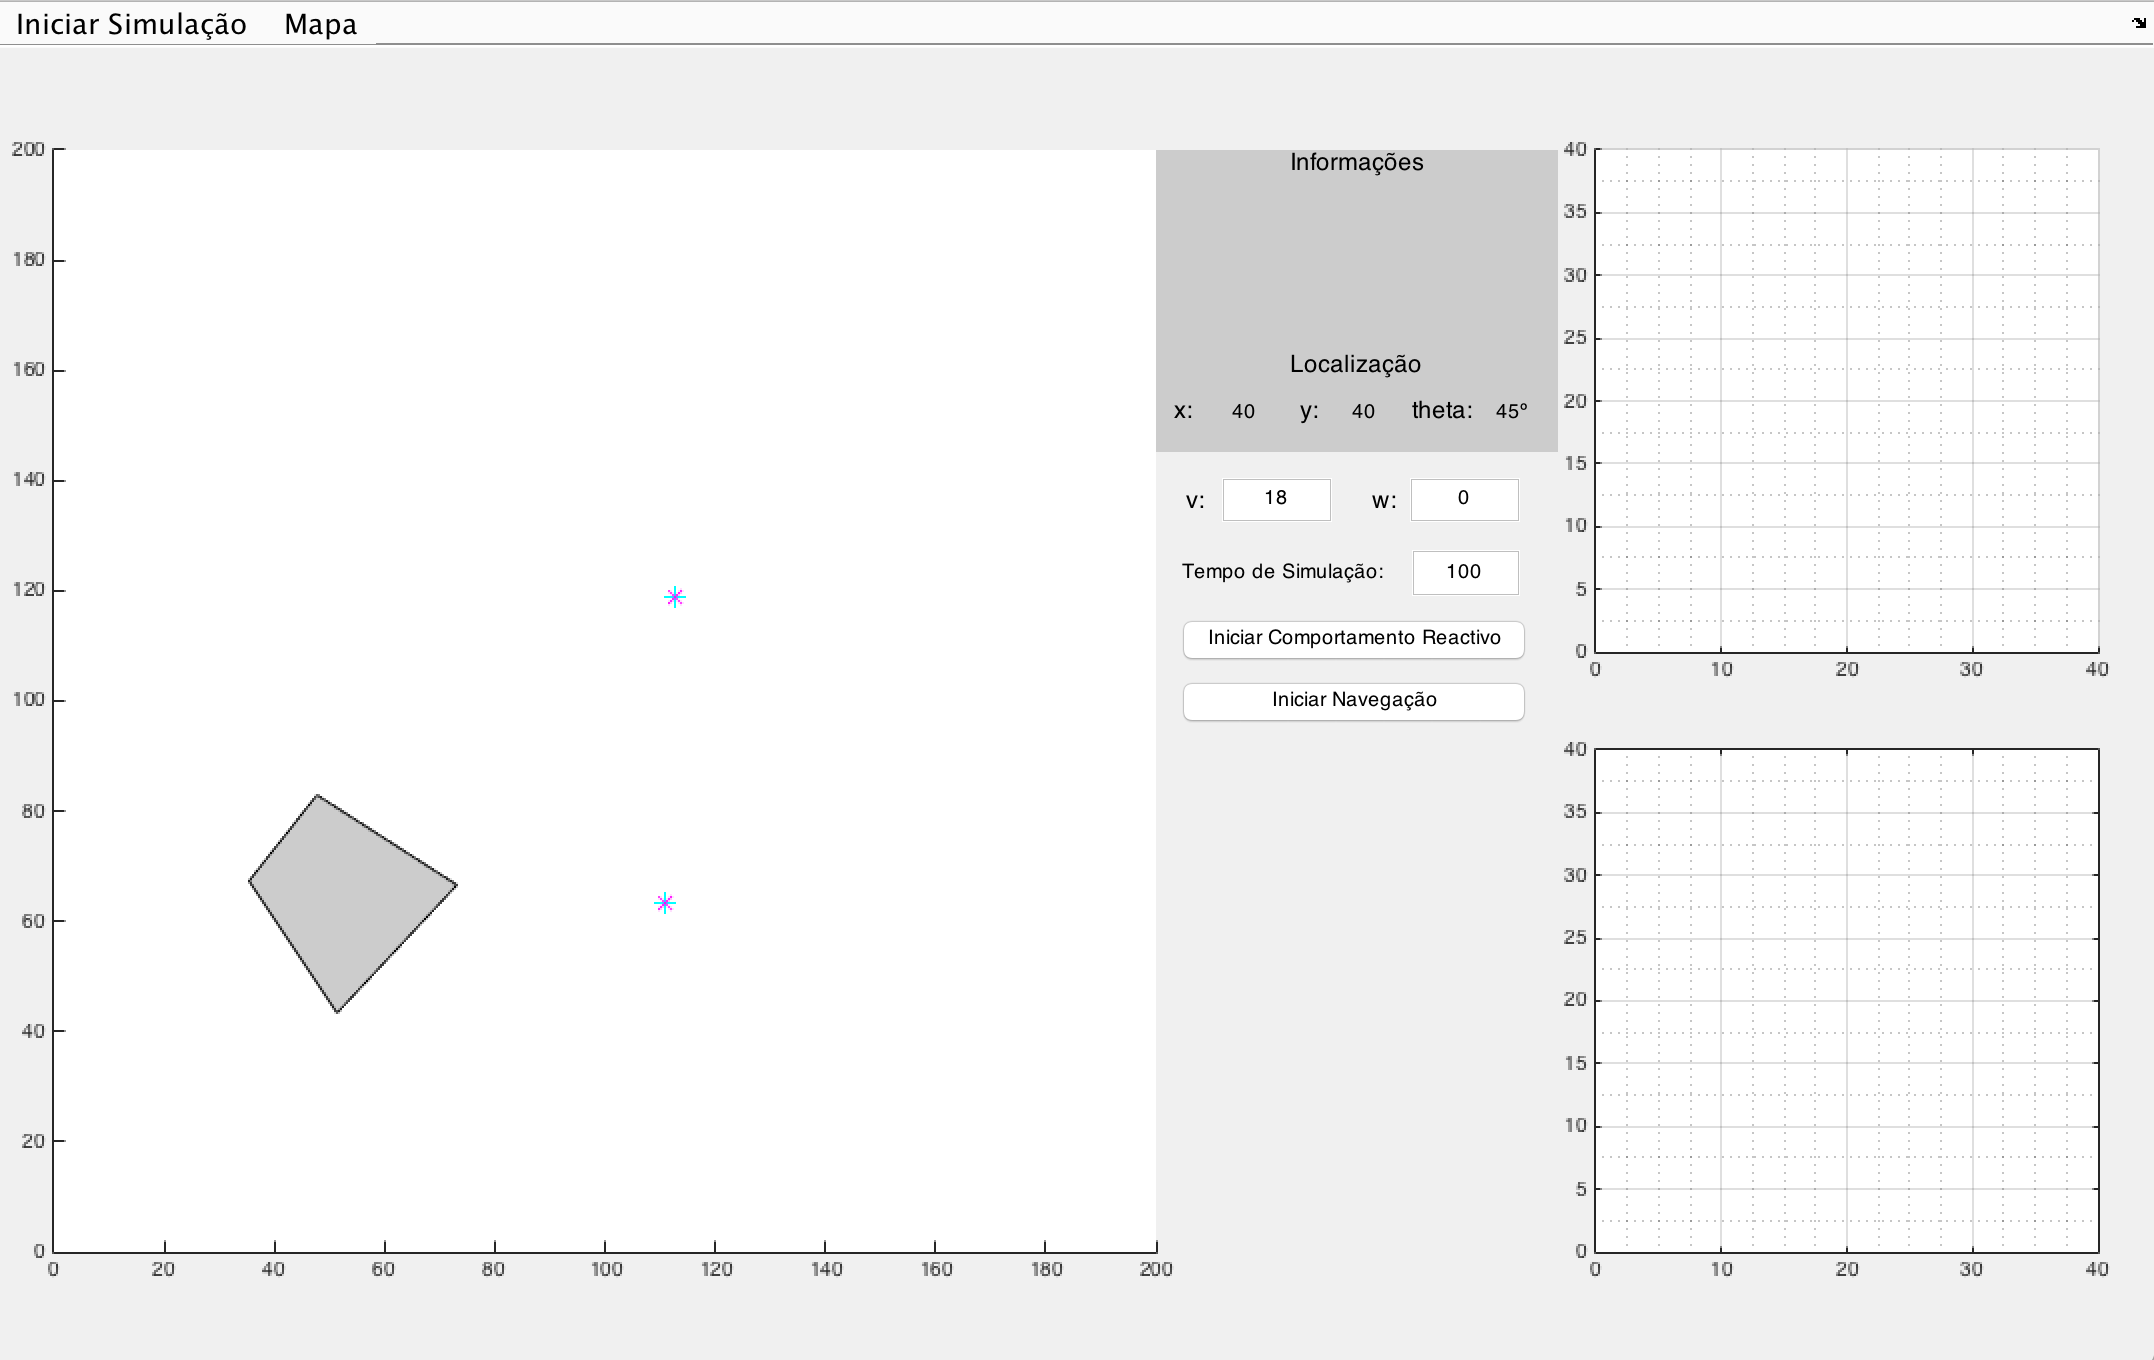
\includegraphics[width=90mm,scale=0.2]{img2.png}
\caption{Captura do simulador no momento de criar um mapa.}\label{fig:fig4}
\end{figure}



%-------------------------------------------------------------------------
\subsection{Implementação prática:}
\indent \\ \indent Para este
labwork é pretendido que a plataforma (que mantém as características dos labworks anteriores) seja capaz de se deslocar de um ponto inicial para um ponto final sem conhecimento prévio do mapa (independentemente da existência de obstáculos), a plataforma apenas não conseguirá atingir o seu objectivo caso exista um mínimo local. Para que a plataforma consiga chegar ao objectivo é criado um mapa de pontencial atractivo em função do ponto destino e um mapa de potencial repulsivo em função da presença de obstáculos, o mapa de ocupação que utiliza o algoritmo desenvolvido por \textbf{Sebastian Thrun} continua a ser utilizado na detecção de obstáculos. \\ \indent Posteriormente ao atingir o ponto objectivo a plataforma deverá regressar ao ponto incial, agora com conhecimento do mapa já percorrido. \\ \indent A plataforma deve como objectivo final navegar entre diversos pontos.




\subsubsection{Funções:}

\indent \\ \indent Com a introdução dos mapas de atracção e repulsão e com a introdução de um novo tipo de navegação houve necessidade de criar e alterar algumas funções novas.
\begin{itemize}


\item \textbf{actualizaGrelhaPotencialObstaculos.m:} -- Esta função tem como parâmetros de entrada \textbf{(matrizOcupado,grelhaPotencialObstaculosAnterior)}.
\begin{itemize}
\item \textbf{matrizOcupado} - matriz de ocupação com o mapa de ocupação determinado com o algoritmo de \textbf{Sebastian Thrun}. 
\item \textbf{grelhaPotencialObstaculosAnterior} - Grelha que inclui o mapa com o potencial reactivo anterior.
\end{itemize}
Esta função, actualizada, vai calcular o potencial repulsivo com base nos valores de anteriores e nos valores da \textbf{matriz ocupado} como é descrito nas fórmulas apresentadas em \ref{fig:fig6}. 


 
  \item \textbf{criaGrelhaPotencial.m:} -- Esta função cria as grelhas de potencial repulsivo.
  \item \textbf{criaGrelhaPotencialDestino.m:} -- Esta função cria as grelhas de potencial atractivo.
  \item \textbf{desenhaGrelhaPotencial.m:} -- Esta função desenha a grelha de potencial final (soma da grelha de potencial atractivo com a grelha de potencial repulsivo).
  \item \textbf{calcParamMovimento.m:} -- Esta função tem como parâmetros de entrada \textbf{(matrizPotencial,x,y,theta)} .
  \begin{itemize}
\item \textbf{matrizPotencial} - matriz com a soma das grelhas de potencial atractivo e repulsivo. 
\item \textbf{x,y} - Coordenadas x,y da plataforma.
\item \textbf{theta} - Orientação da plataforma.
\end{itemize}
Esta função vai utilizar a informação da posição da plataforma para determinar o ângulo de rotação em relação ao destino. Após este cálculo esta função desloca a plataforma em direção ao ponto objectivo.
  
  
   \textbf{(matrizOcupadoAnterior,theta,rho,m,n,R)}


  
  


\begin{figure}[ht]
\centering
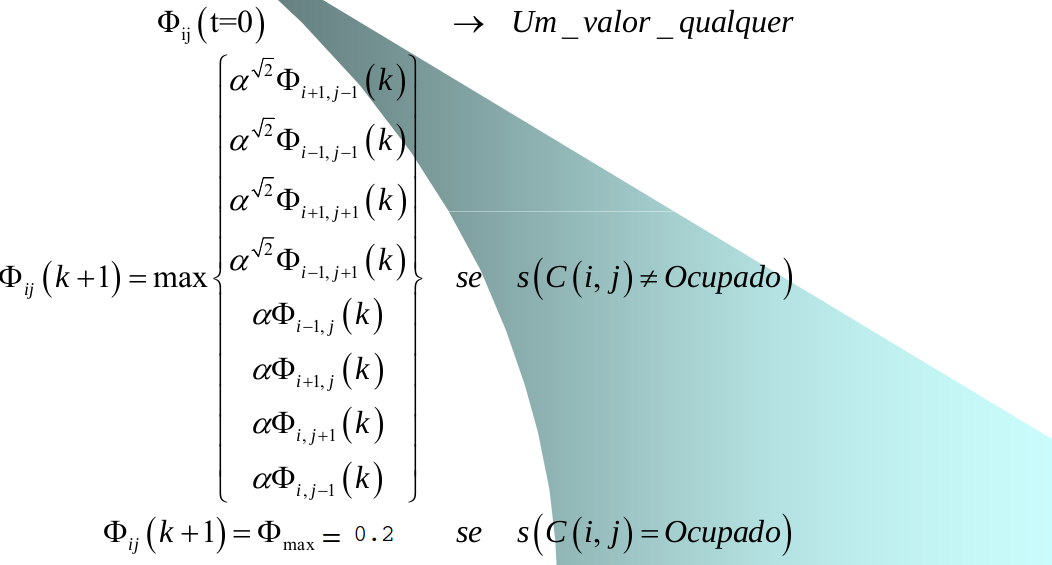
\includegraphics[width=170mm,scale=2]{6.png}
\caption{Cálculo da grelha de potencial repulsivo  .}\label{fig:fig6}
\end{figure}


\newpage

  

  
 
\end{itemize}

\subsection{Análise de Resultados:}
 \indent O simulador foi testado em diferentes mapas.

\begin{figure}[ht]
\centering
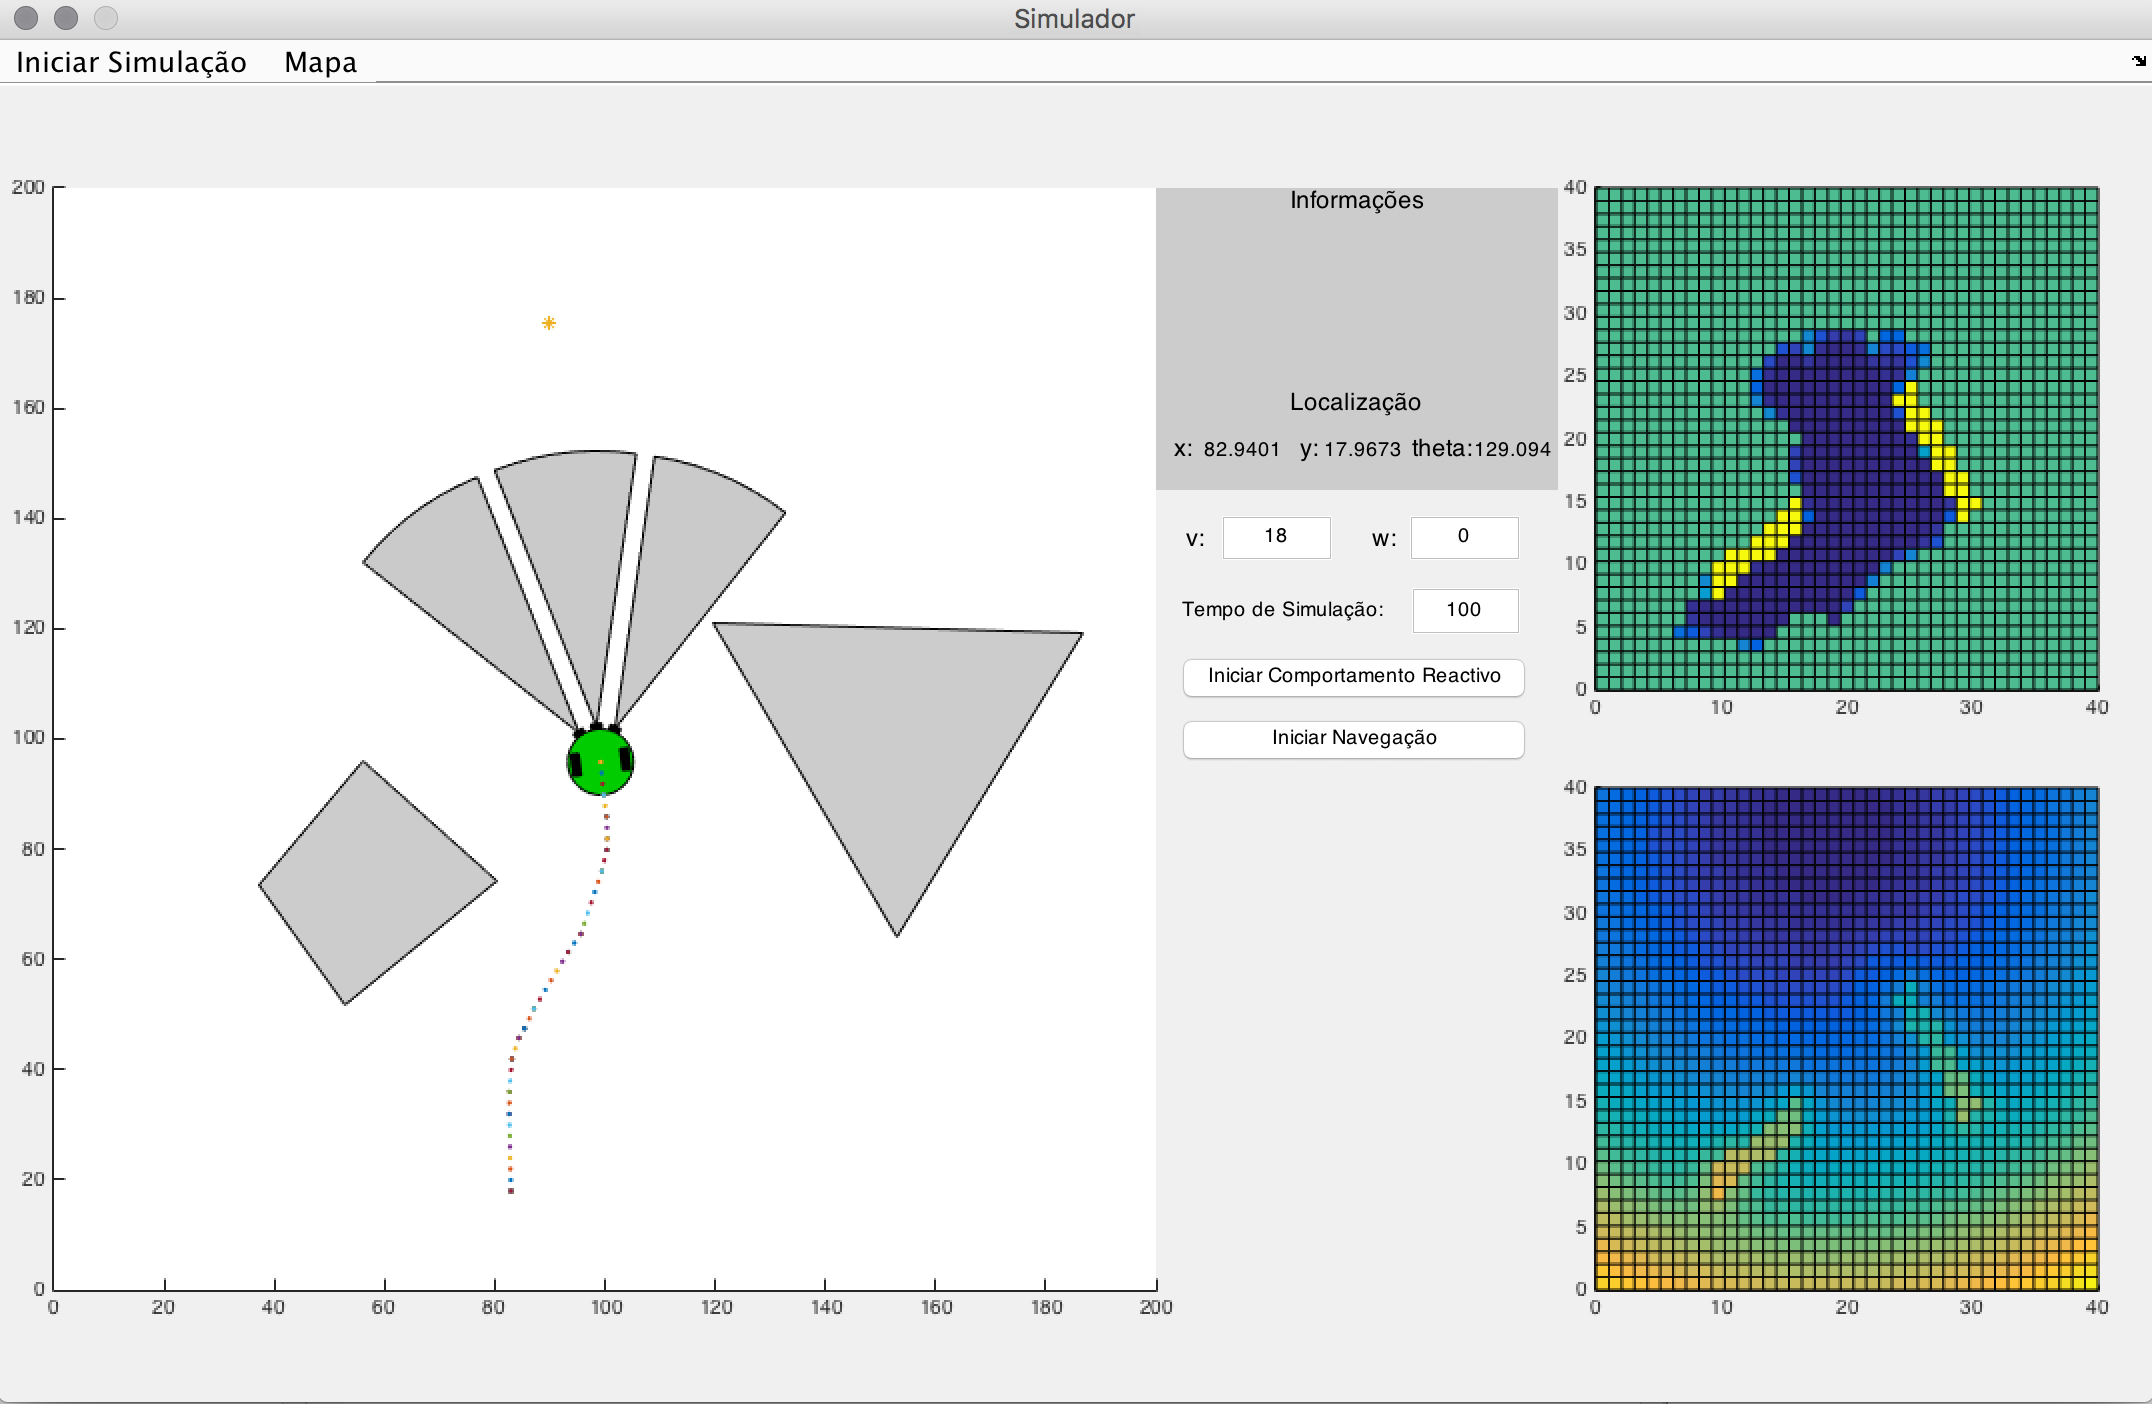
\includegraphics[width=90mm,scale=0.2]{img3.png}
\caption{Captura do simulador no durante o percurso . Mapa de ocupação e de potencial à direita.}\label{fig:fig4}
\end{figure}


\begin{figure}[H]
\centering
\subfloat[]{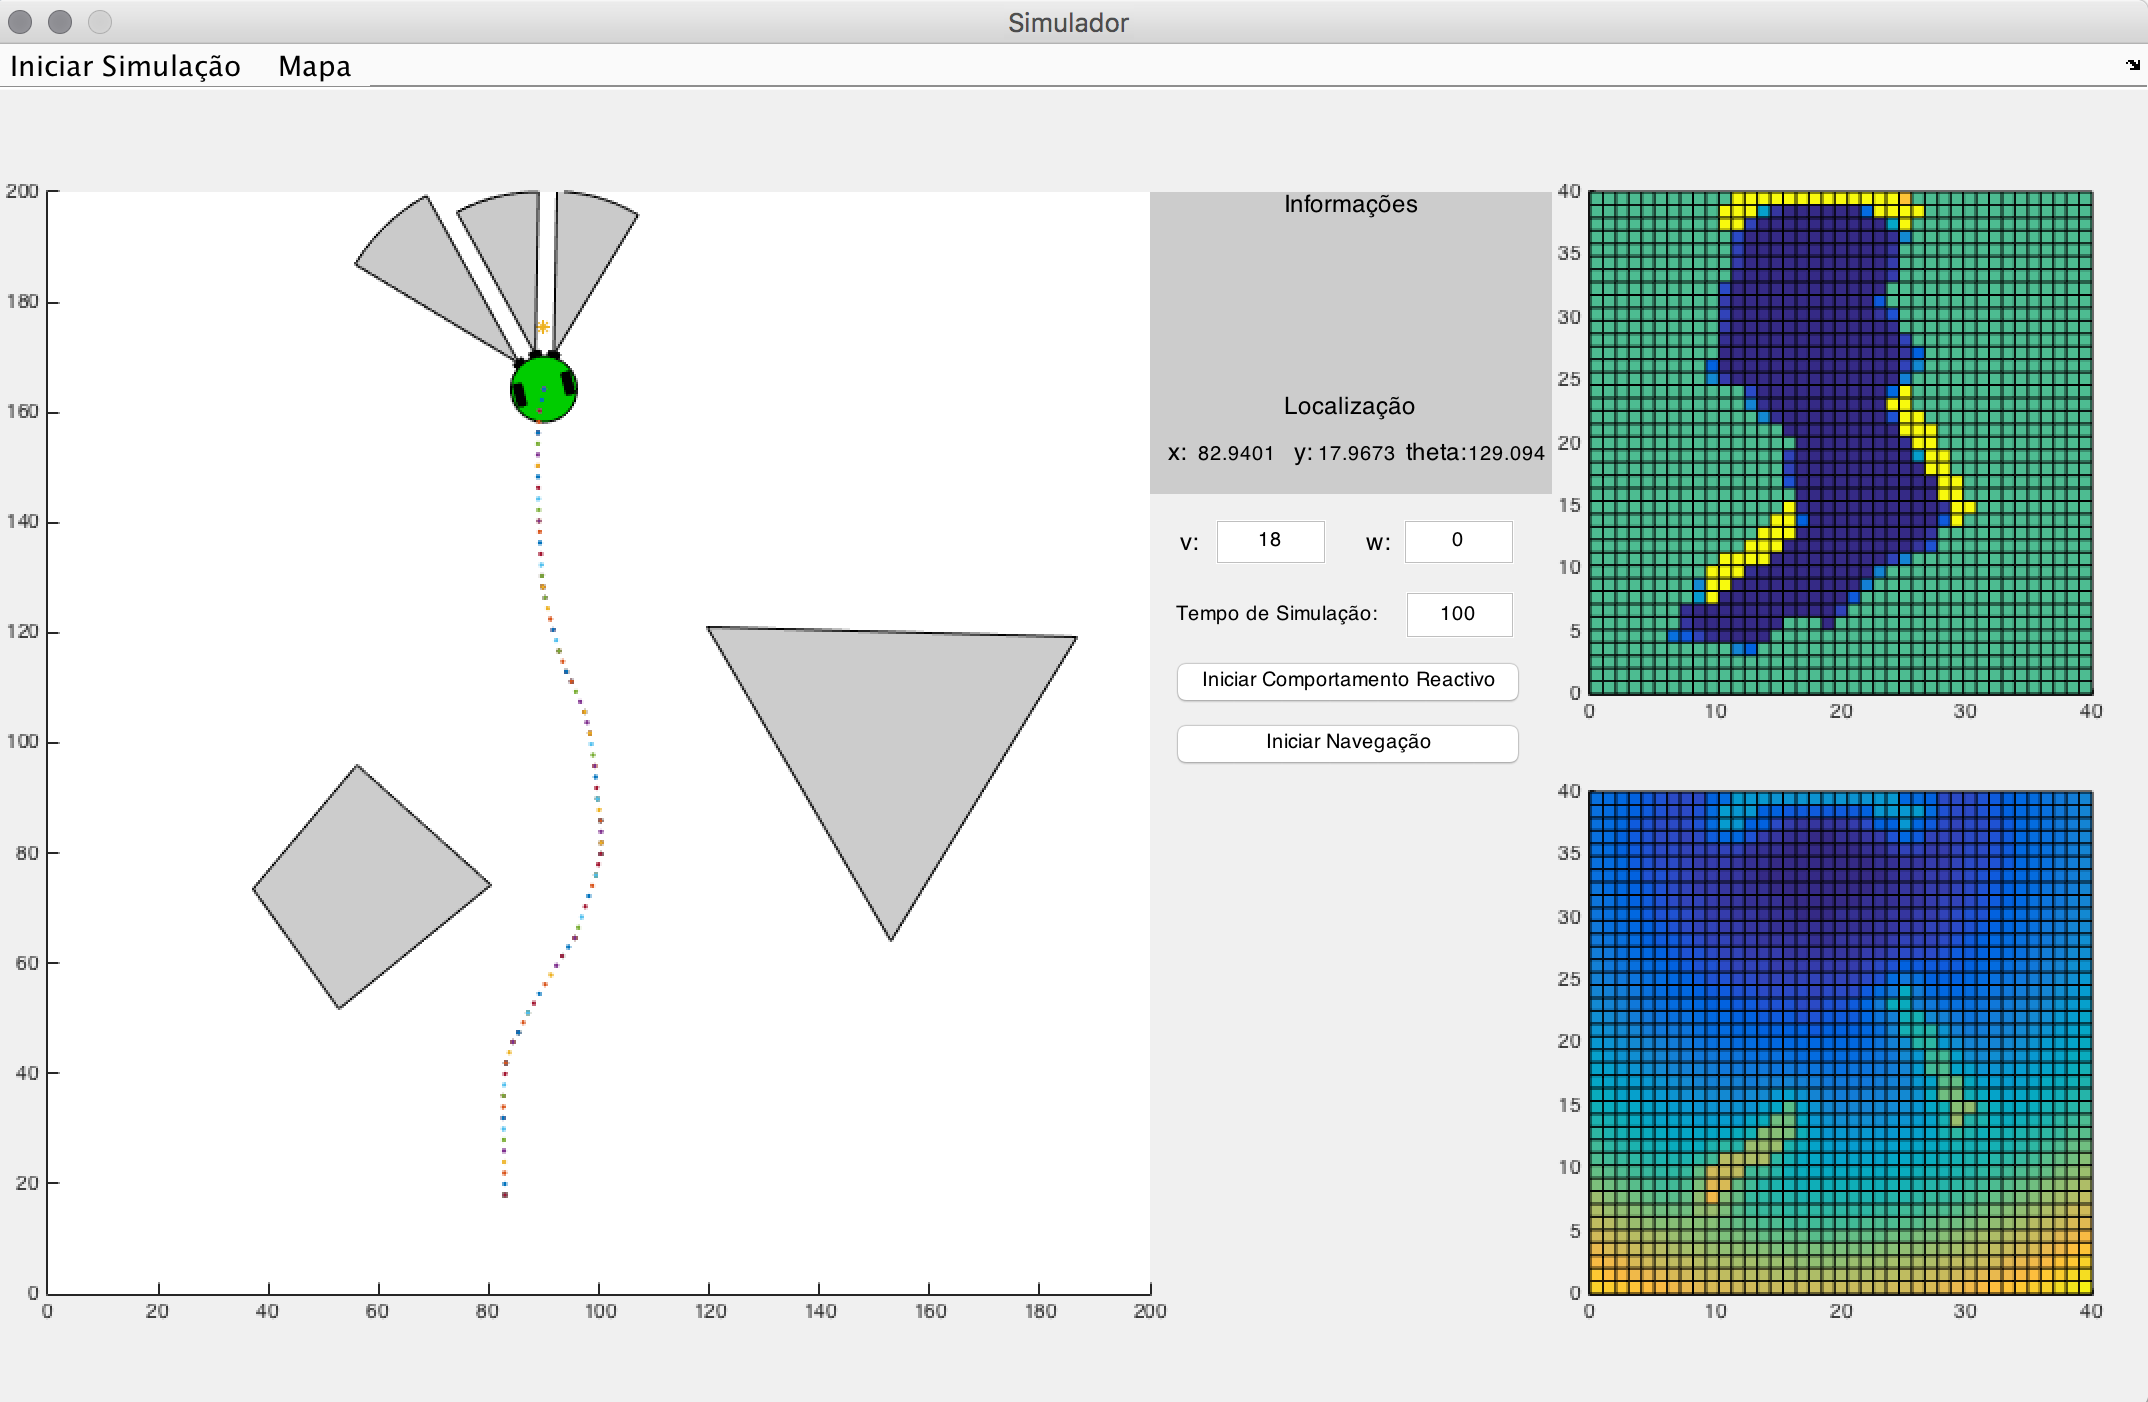
\includegraphics[width=3.1in]{img4.png}} 
\subfloat[]{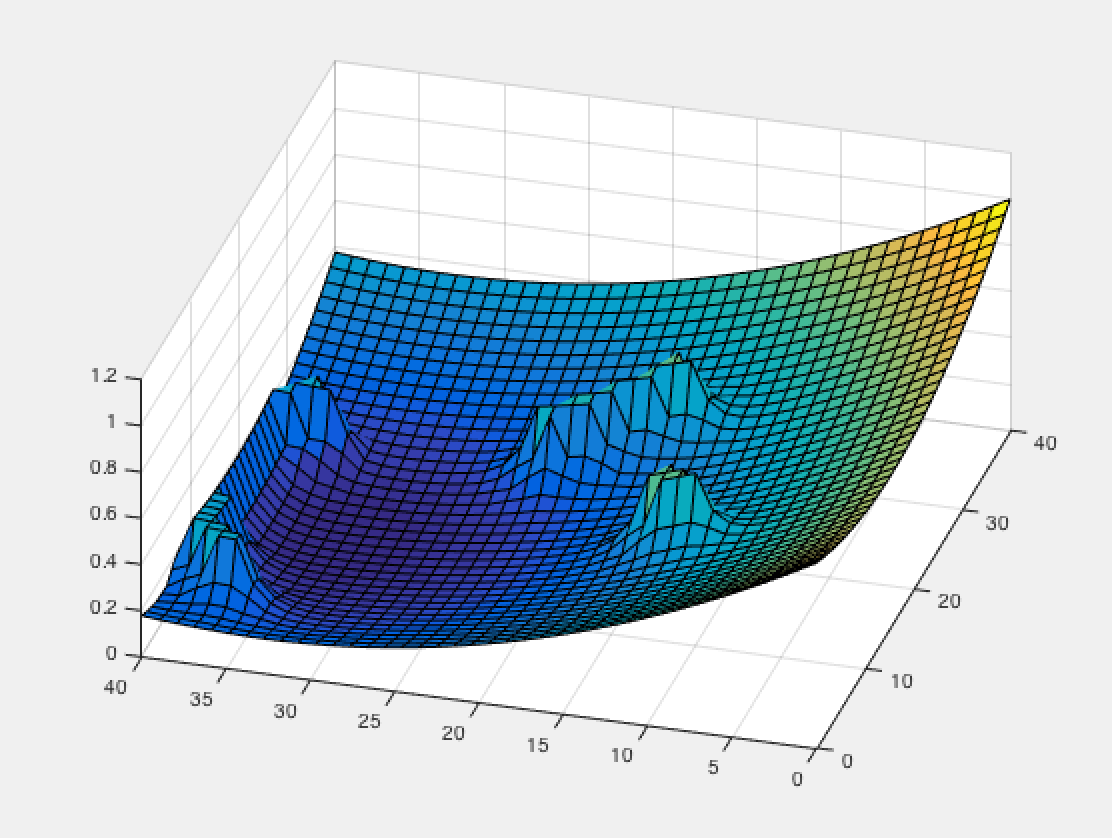
\includegraphics[width=3.1in]{img5.png}}
\caption{Captura do final da simulação (esquerda) e do mapa de potencial final . } 

\begin{figure}[H]
\centering
\subfloat[]{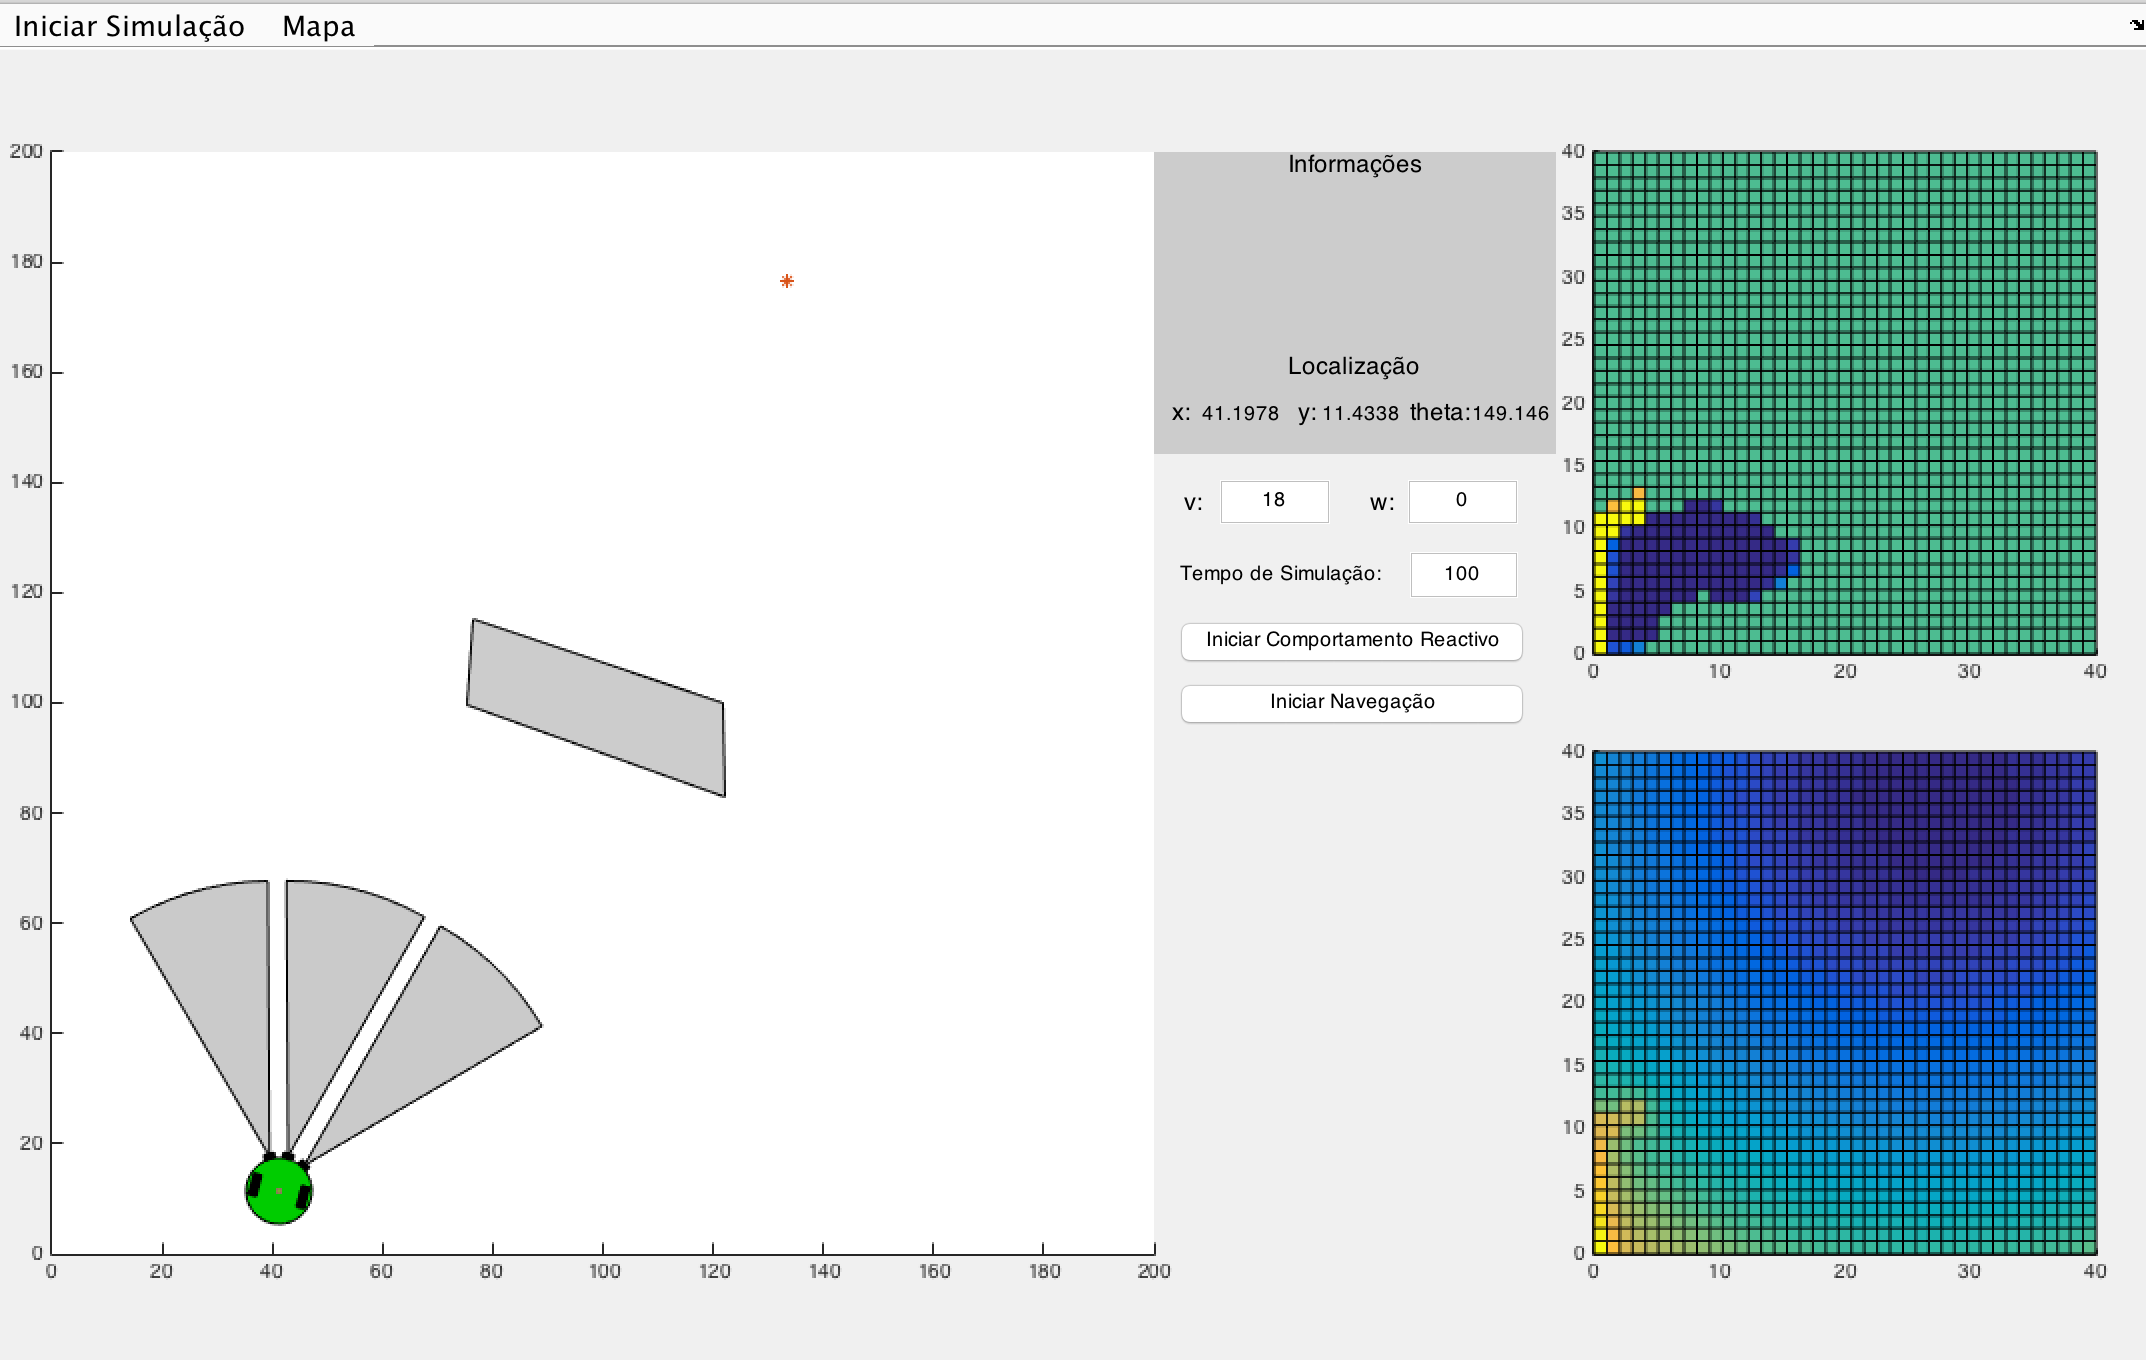
\includegraphics[width=3.1in]{img6.png}} 
\subfloat[]{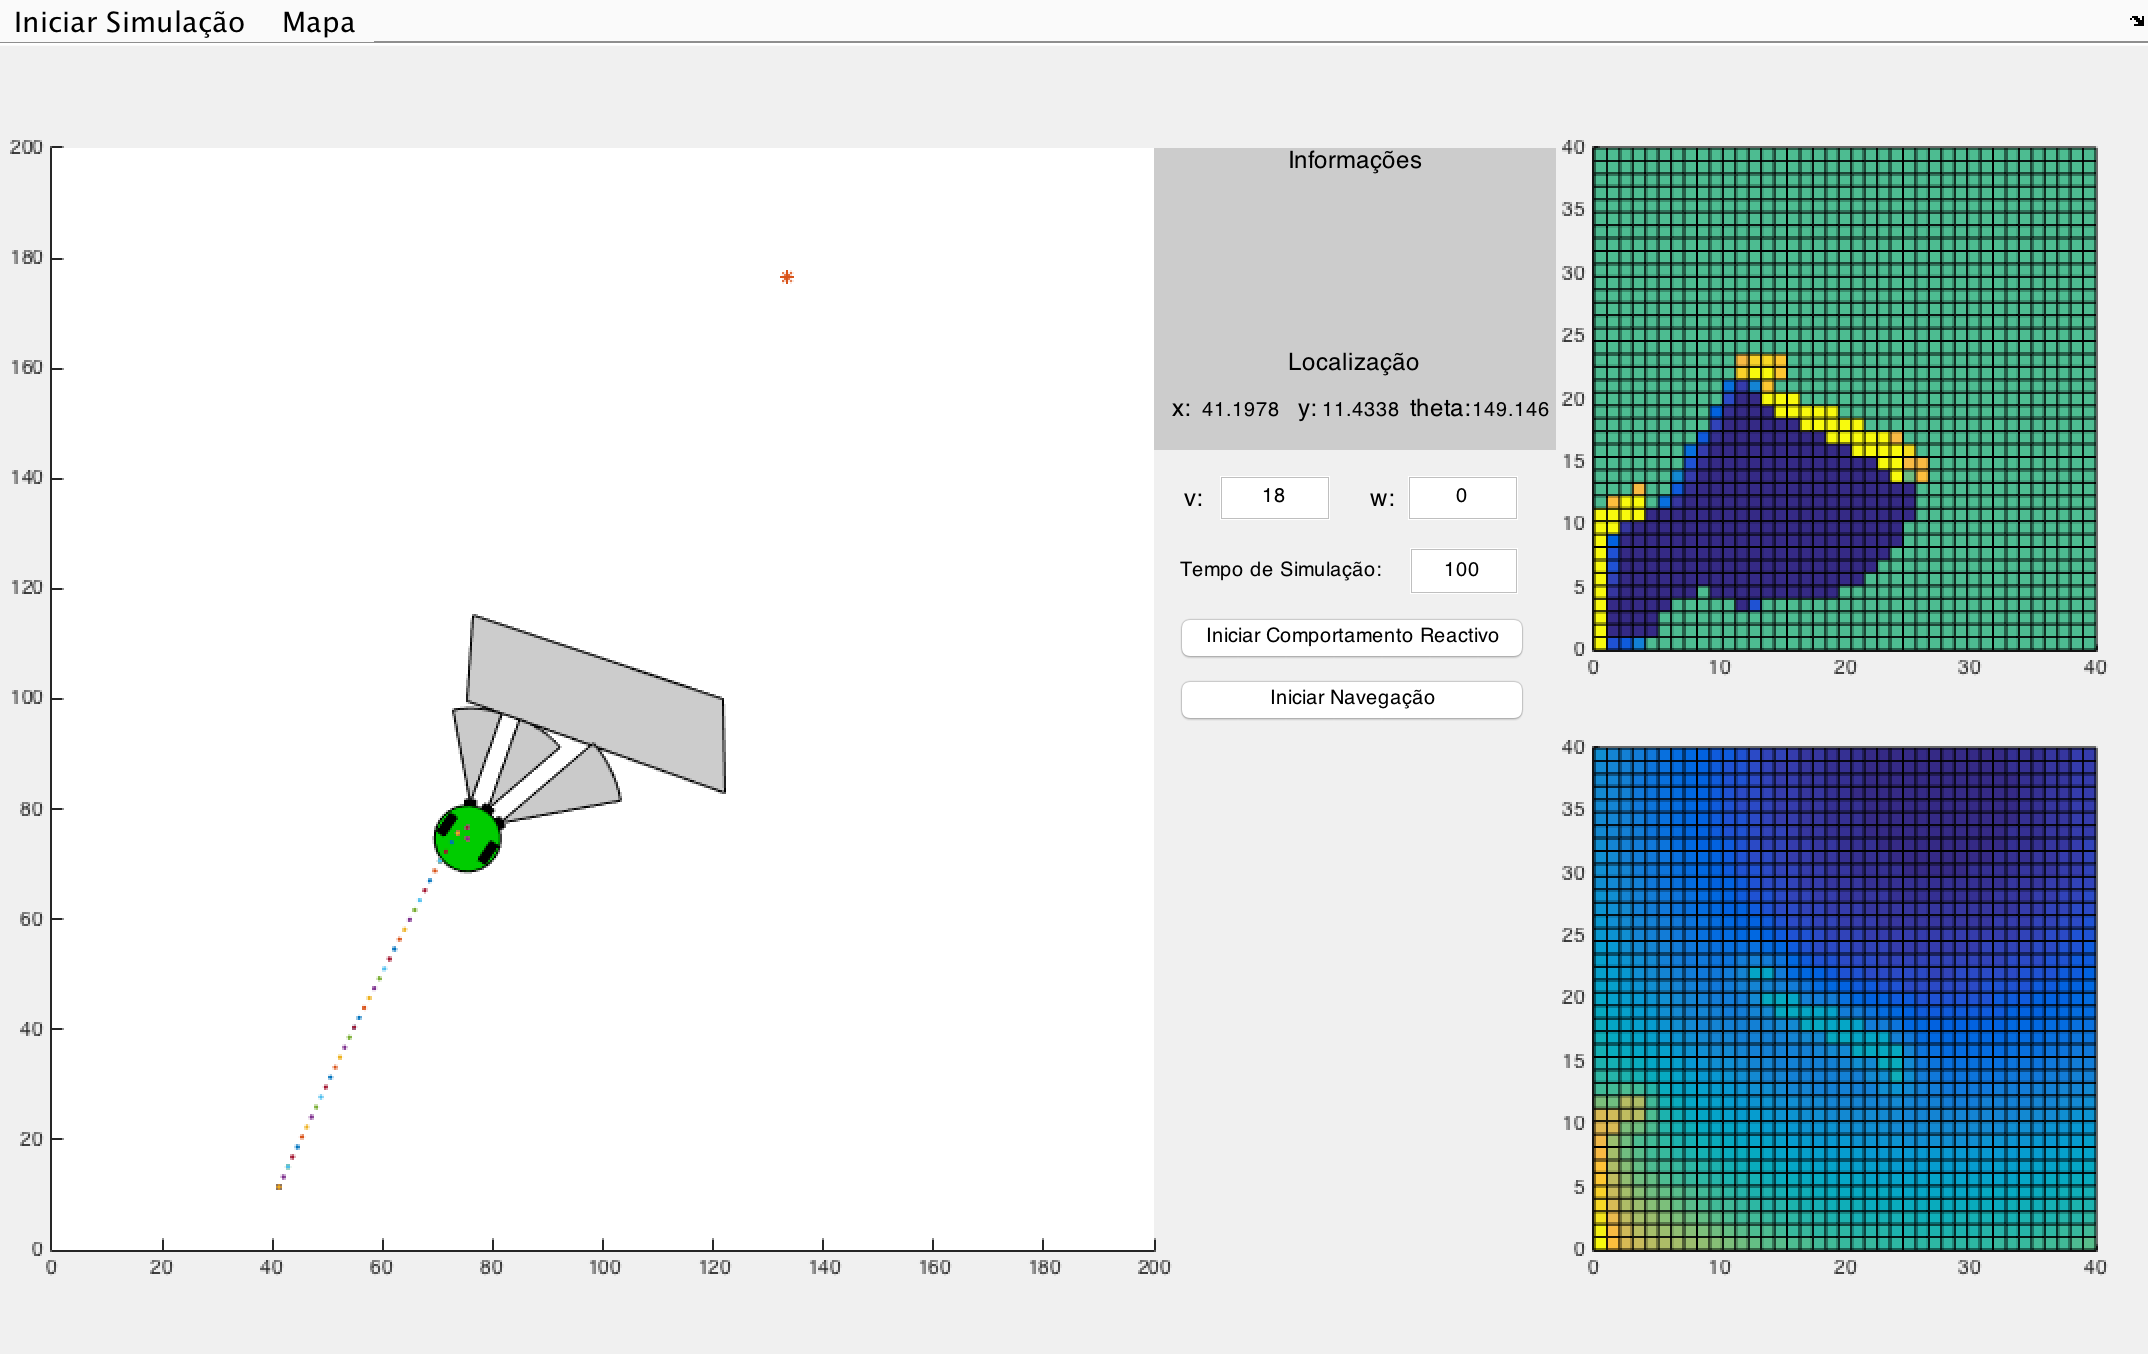
\includegraphics[width=3.1in]{img7.png}}
\caption{Simulação com um mapa diferente. } 
\label{fig:EcUND} 
\end{figure}

\label{fig:EcUND} 
\end{figure}
\begin{figure}[H]
\centering
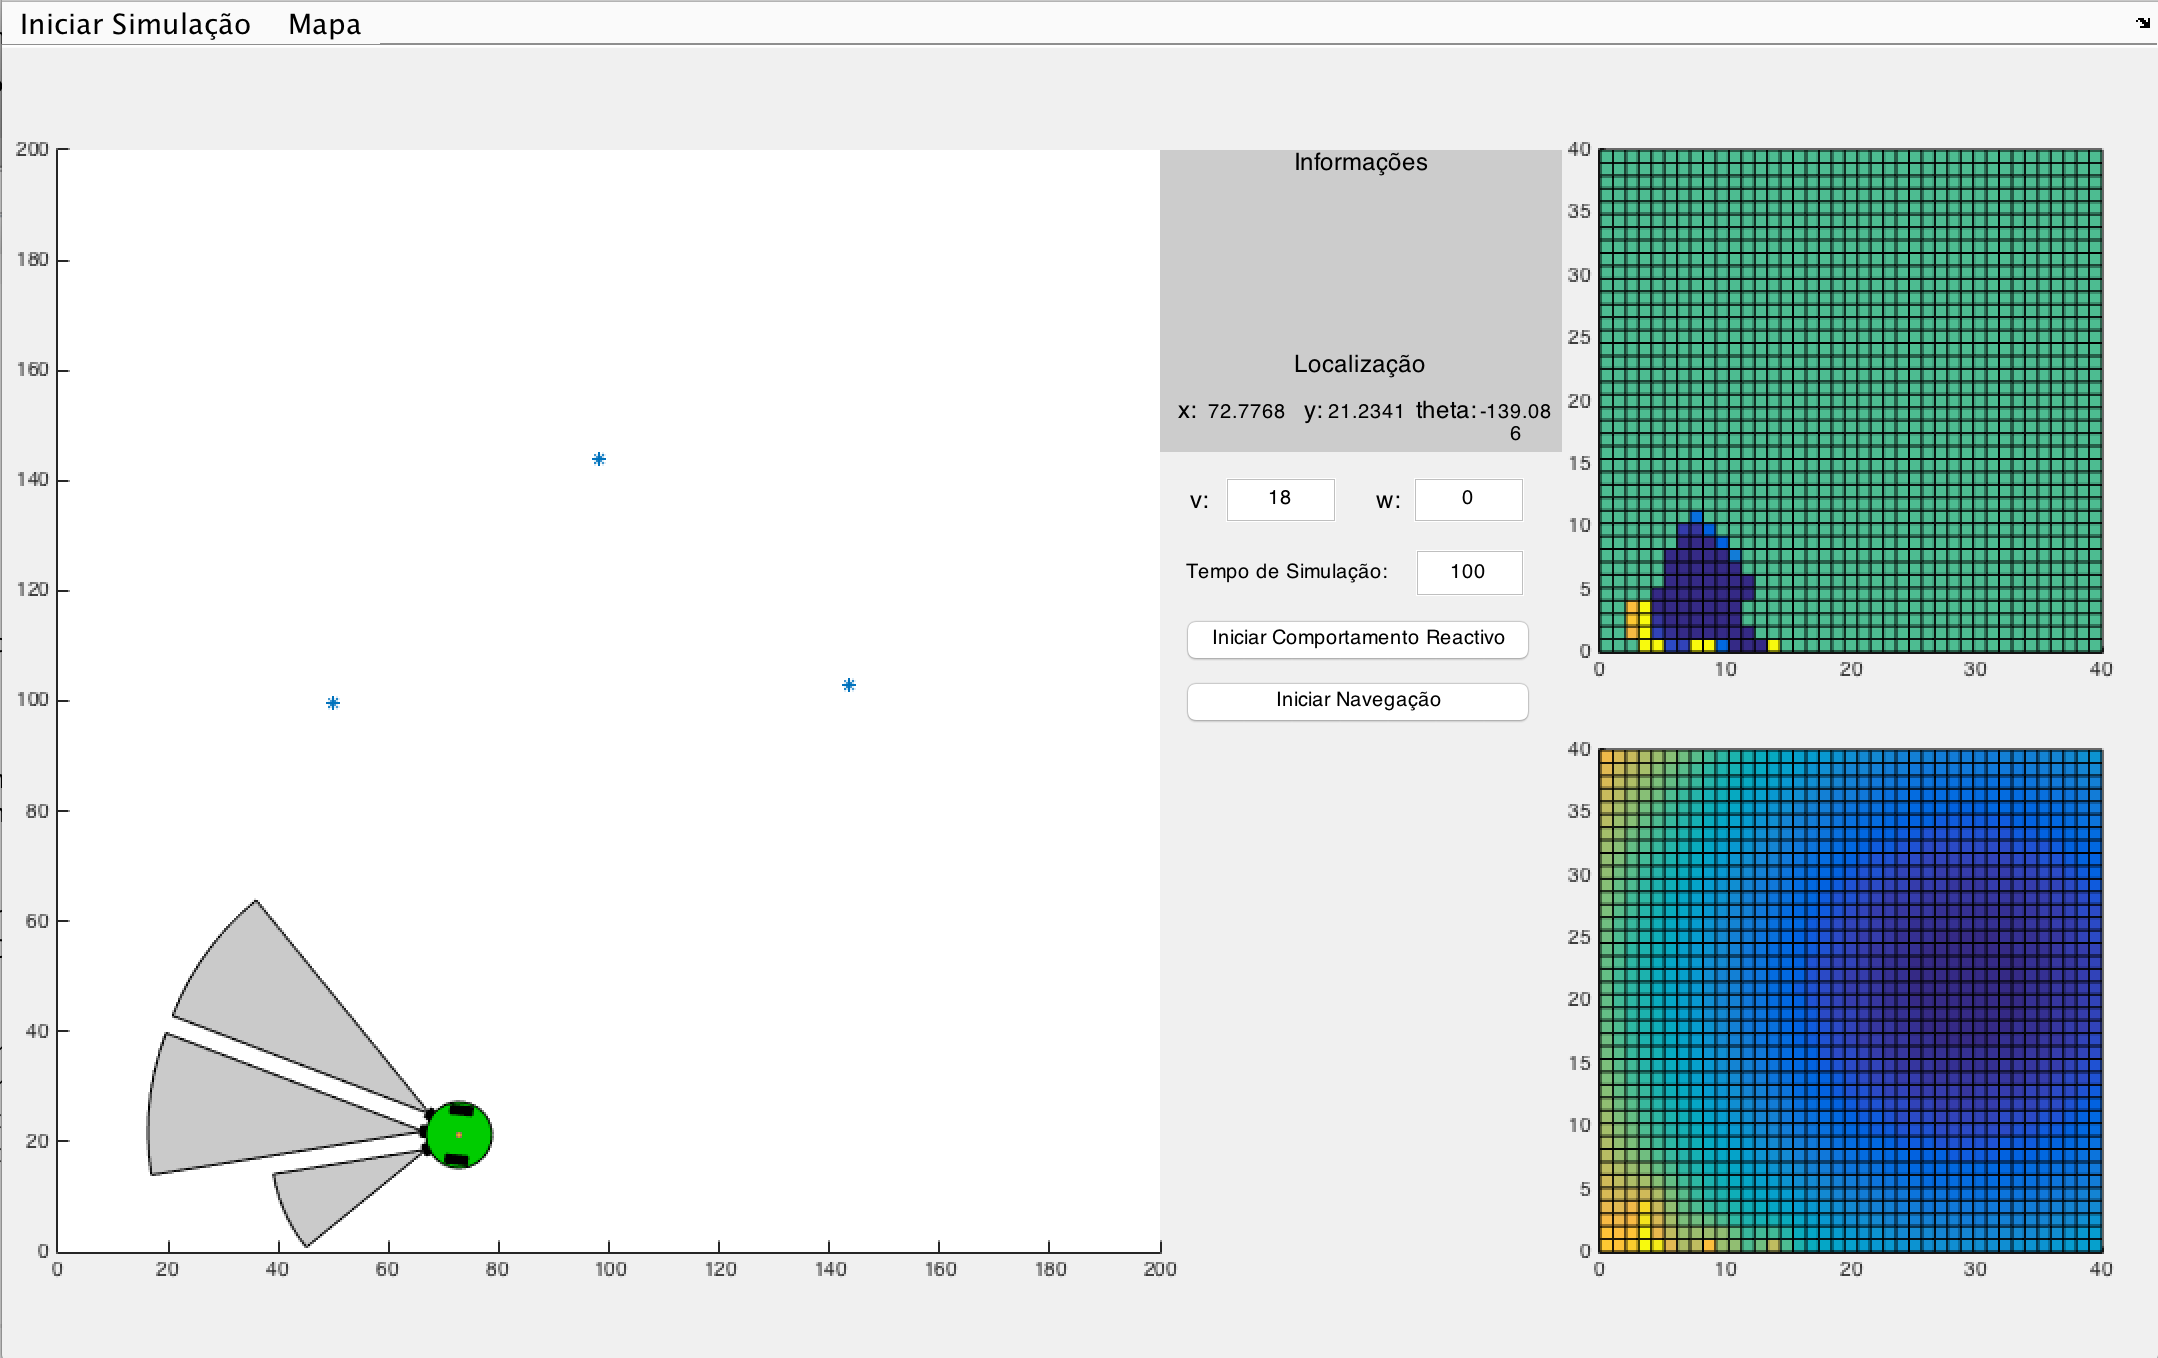
\includegraphics[width=90mm,scale=0.2]{img8.png}
\caption{Navegação ponto a ponto.}\label{fig:fig4}
\end{figure}

\begin{figure}[H]
\centering
\subfloat[]{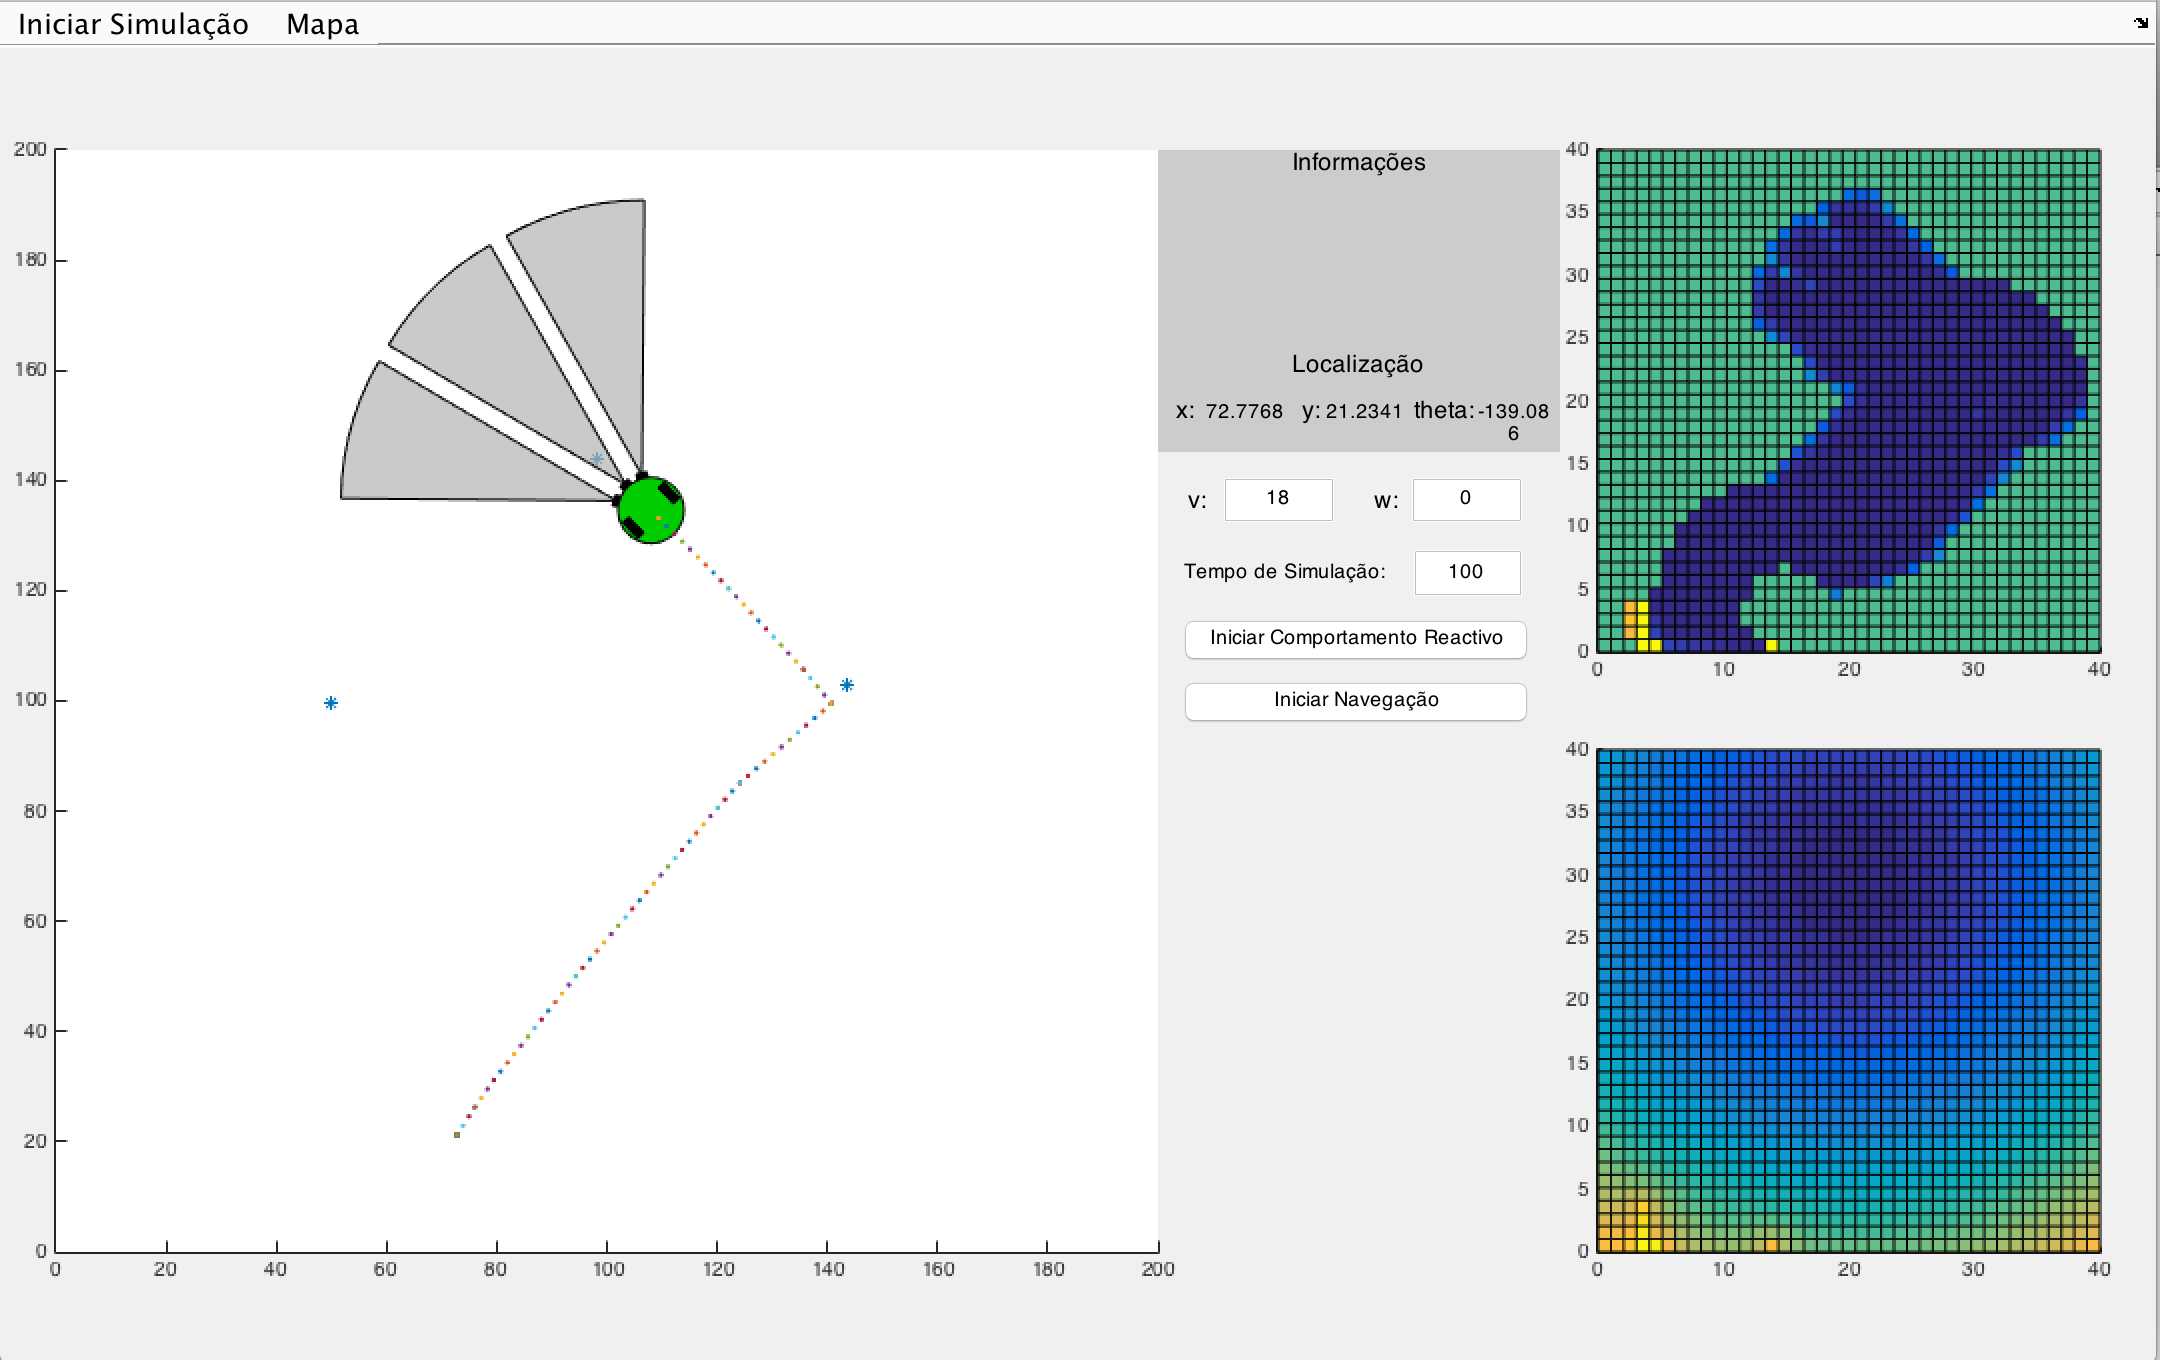
\includegraphics[width=3.1in]{img10.png}} 
\subfloat[]{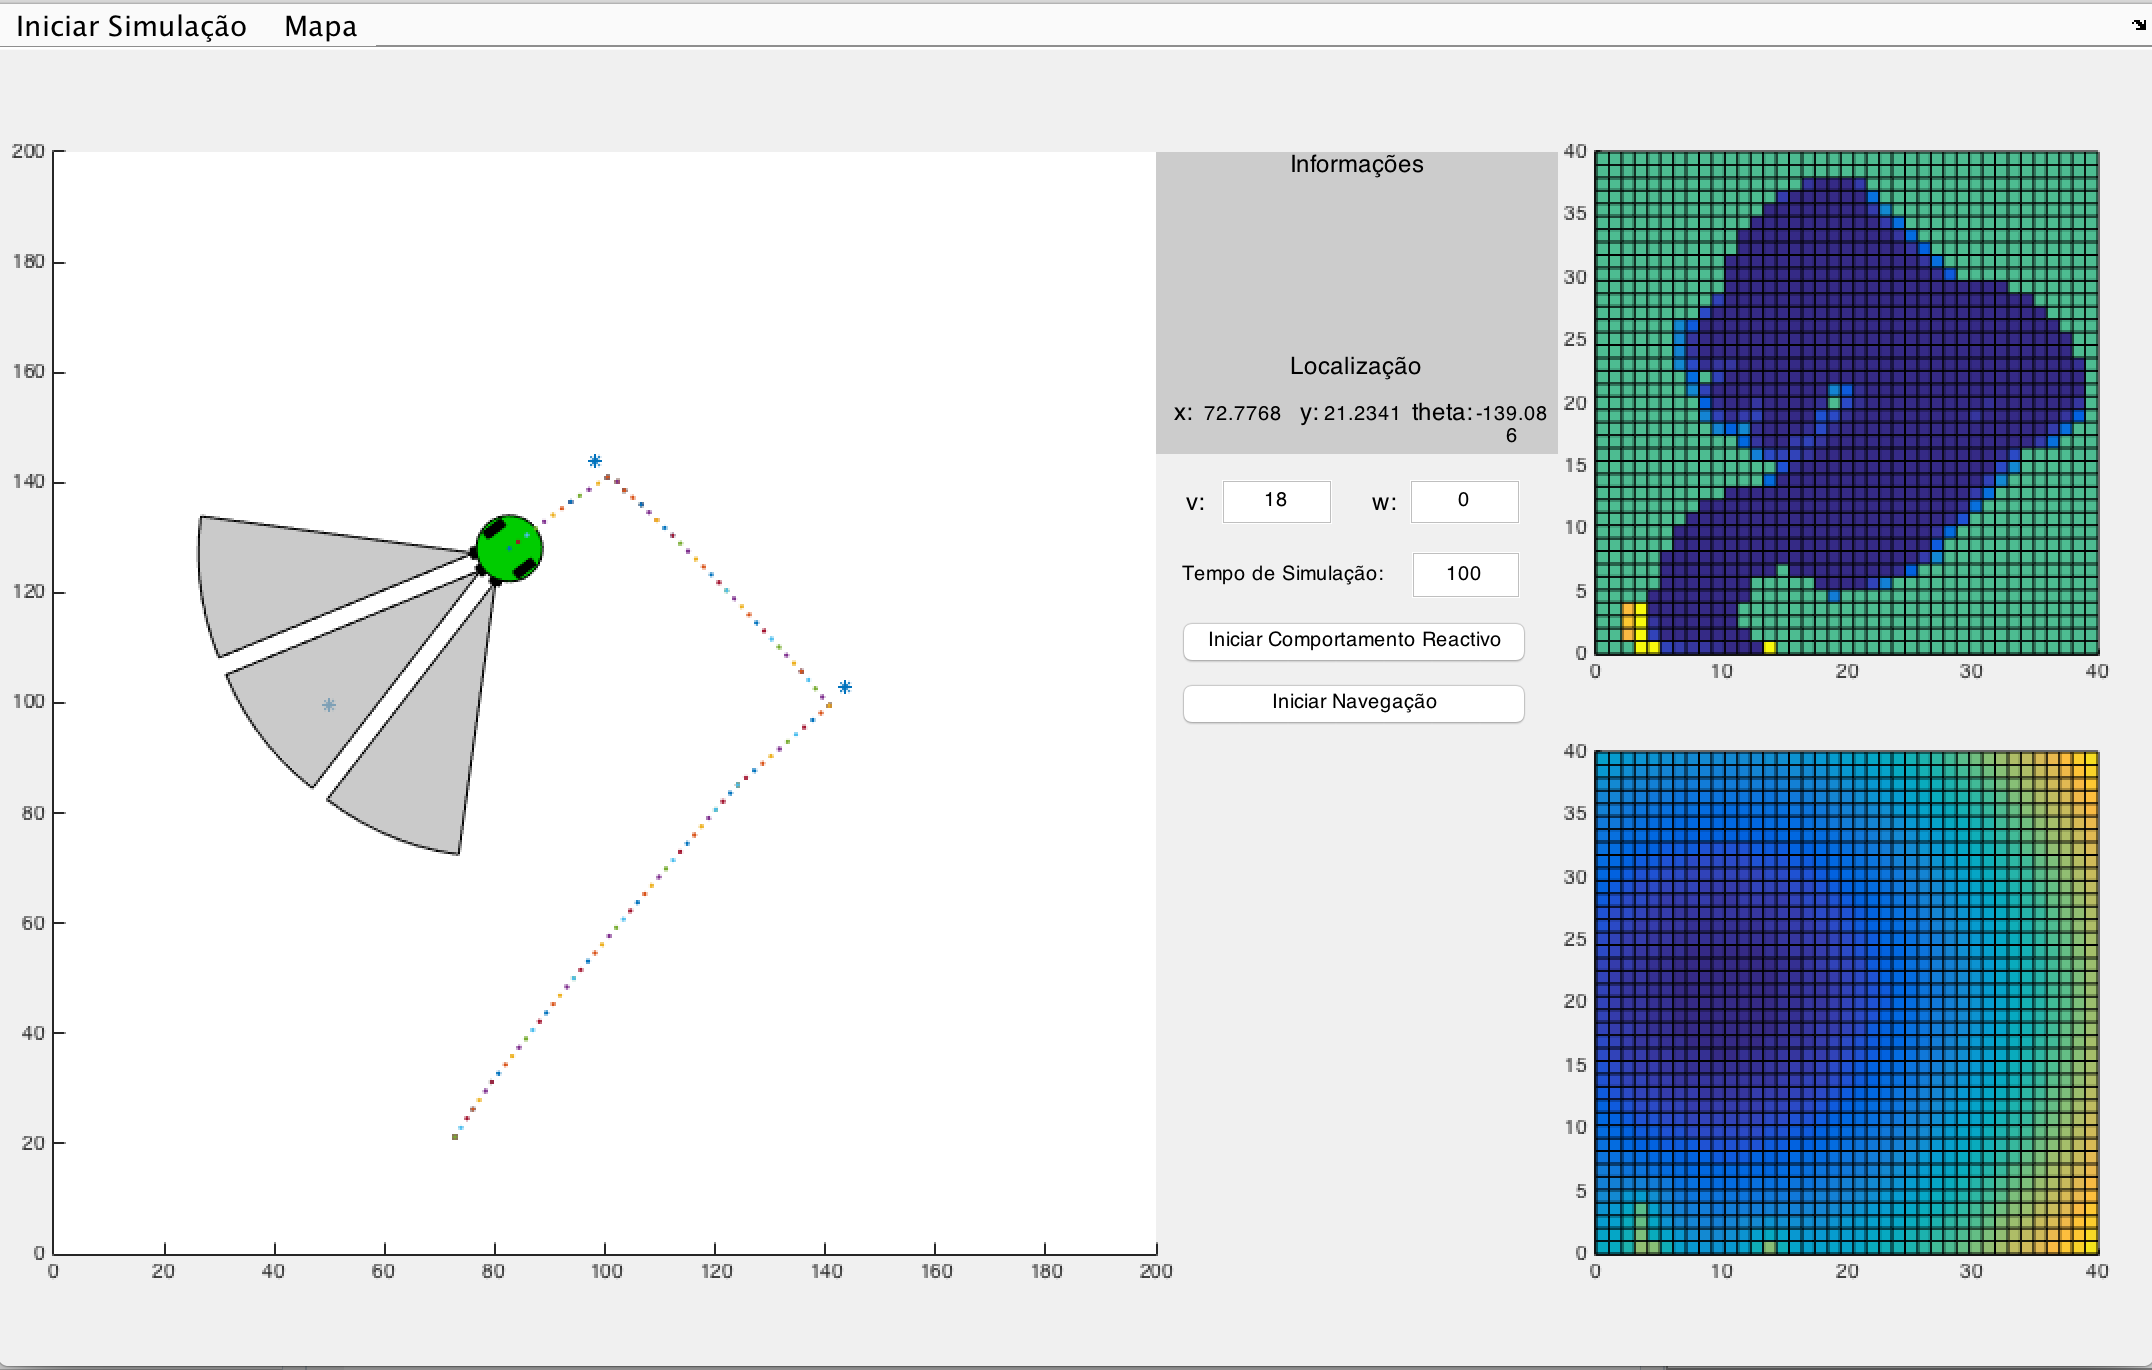
\includegraphics[width=3.1in]{img11.png}}
\caption{Navegação ponto a ponto . } 
\label{fig:EcUND} 
\end{figure}

Verifica-se consegue convergir para diferentes pontos independentemnente da existência de obstáculos desde que não existam mínimos locais.




% \section{References}
%\phantomsection \addcontentsline{toc}{section}{\referencesname}
%\bibliographystyle{unsrt}
%\bibliographystyle{IEEEtran}
%\bibliography{biblio}
% \nocite{*}


% \newpage
% % \thispagestyle{empty}
% \null

% \cleardoublepage
%\listoftodos




\end{document}